\documentclass{hitec}
\usepackage{graphicx}
\usepackage{lscape}
\usepackage{longtable}
\usepackage{subcaption} 
\usepackage[space]{grffile}
\usepackage{pdfpages}
\usepackage{listings}
\usepackage{amsmath}
\definecolor{mygray}{rgb}{0.5,0.5,0.5}
\lstset{  breaklines=true, numbers=left, numberstyle=\tiny\color{mygray}, keepspaces=true }

%https://tex.stackexchange.com/questions/182467/including-eps-figure-in-pdflatex
\usepackage{epsfig}

\usepackage{siunitx} %https://tex.stackexchange.com/questions/413312/how-to-put-angstrom/413317

\usepackage{titlesec}
\usepackage{hyperref}
\usepackage{enumitem} %https://www.latex-tutorial.com/tutorials/lists/

%\usepackage{wasysym}
\usepackage{mathabx}

% https://shantoroy.com/latex/add-subfig-in-latex/
\usepackage{caption}
\usepackage{subcaption}

\usepackage{pgfplots} % https://www.tug.org/TUGboat/tb31-1/tb97wright-pgfplots.pdf

\usepackage{listings} % https://en.wikibooks.org/wiki/LaTeX/Source_Code_Listings

\usepackage[section]{placeins} % page 117 of Latex cookbook

\usepackage{natbib}

\usepackage{xcolor}
\hypersetup{
	colorlinks,
	linkcolor={blue!50!black},
	citecolor={blue!50!black},
	urlcolor={blue!80!black}
}

\usepackage{color, colortbl}
\definecolor{DSNE-Blue}{rgb}{0.773, 0.848, 0.941}
\definecolor{DSNE-Gray}{rgb}{0.848, 0.848, 0.848}

\titleclass{\subsubsubsection}{straight}[\subsection]

\newcounter{subsubsubsection}[subsubsection]
\renewcommand\thesubsubsubsection{\thesubsubsection.\arabic{subsubsubsection}}
\renewcommand\theparagraph{\thesubsubsubsection.\arabic{paragraph}} % optional; useful if paragraphs are to be numbered

\titleformat{\subsubsubsection}
{\normalfont\normalsize\bfseries}{\thesubsubsubsection}{1em}{}
\titlespacing*{\subsubsubsection}
{0pt}{3.25ex plus 1ex minus .2ex}{1.5ex plus .2ex}

\makeatletter
\renewcommand\paragraph{\@startsection{paragraph}{5}{\z@}%
	{3.25ex \@plus1ex \@minus.2ex}%
	{-1em}%
	{\normalfont\normalsize\bfseries}}
\renewcommand\subparagraph{\@startsection{subparagraph}{6}{\parindent}%
	{3.25ex \@plus1ex \@minus .2ex}%
	{-1em}%
	{\normalfont\normalsize\bfseries}}
\def\toclevel@subsubsubsection{4}
\def\toclevel@paragraph{5}
\def\toclevel@paragraph{6}
\def\l@subsubsubsection{\@dottedtocline{4}{7em}{4em}}
\def\l@paragraph{\@dottedtocline{5}{10em}{5em}}
\def\l@subparagraph{\@dottedtocline{6}{14em}{6em}}
\makeatother

\setcounter{secnumdepth}{4}
\setcounter{tocdepth}{4}


\title{SLS Booster Radiation Environment}
\author{Anthony M. DeStefano}
\company{NASA, MSFC, EV44}
\confidential{\textbf{-- For internal NASA and partners use only --}}
\usepackage{hyperref} 
\begin{document}
\maketitle
\pagenumbering{roman}

\tableofcontents
\listoffigures
\listoftables
\lstlistoflistings
\newpage



%\section*{Contributing Author List}
%\addcontentsline{toc}{section}{Contributing Author List}



\cleardoublepage
\pagenumbering{arabic}
%%%%%%%%%%%%%%%%%%%%%%%%%%%%%%%%%%%%%%%%%%%%%%%%%%%%%%%%%%%%%%%%%%
%%%%%%%%%%%%%%%%%%%%%%%%%%%%%%%%%%%%%%%%%%%%%%%%%%%%%%%%%%%%%%%%%%
\section{Executive Summary}


\newpage
%%%%%%%%%%%%%%%%%%%%%%%%%%%%%%%%%%%%%%%%%%%%%%%%%%%%%%%%%%%%%%%%%%
%%%%%%%%%%%%%%%%%%%%%%%%%%%%%%%%%%%%%%%%%%%%%%%%%%%%%%%%%%%%%%%%%%
\section{Reproducing DSNE 200 km Tables using CREME96}

The 200 km LET (Linear Energy Transfer) and particle flux environments SLS-SPEC-159 Cross-Program Design Specification for Natural Environments (DSNE) were obtained using the Cosmic Ray Effects on Microelectrons 96 (CREME96\footnote{\url{https://creme.isde.vanderbilt.edu/}}). In this section, DSNE Tables 3.2.13-1 -- 3 are reproduced using the technical notes provided in the DSNE.

For the LET and flux, the \textsf{GTRN} routine is ran using the following options:
\begin{itemize}
	\item 1.C.a. \& 1.C.b. 200 km circular orbit
	\item 1.C.c. 51.6 degrees orbit inclination
	\item 1.C.g. Effective L-shell range: $2.4 \le L \le 2.55$
	\item 2. Stormy magnetic weather conditions
\end{itemize}

\subsection{Linear Energy Transfer (LET)}\label{ssec:LET}

To compute the LET, the \textsf{LETSPEC} routine is used setting the following parameters:
\begin{itemize}
	\item 2. and 3. $Z = 1 \text{ to } 92$
	\item 4. particles $> 0.1 $ MeV/nuc
	\item 5. Silicon target material
\end{itemize}
\begin{figure}[htbp!]
	\centering
	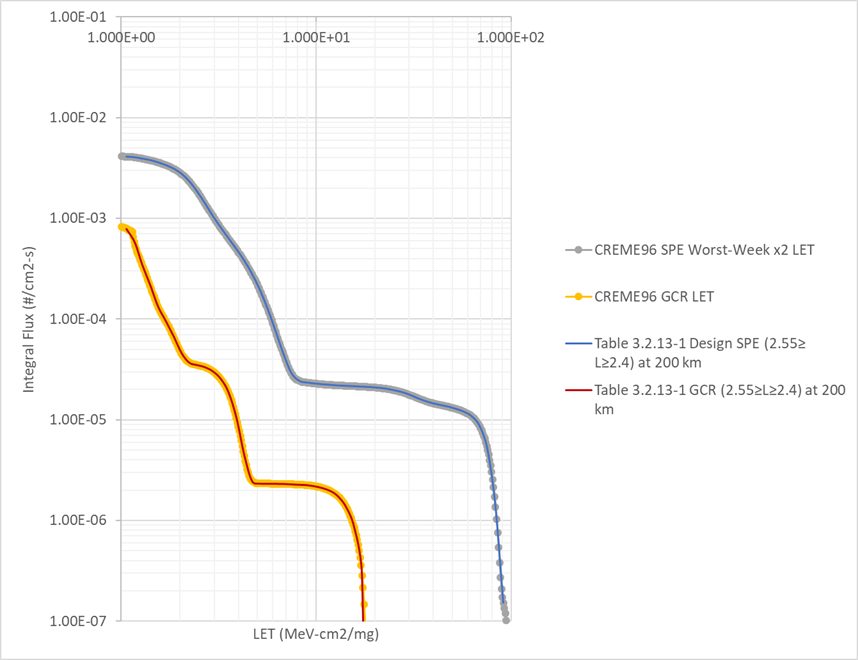
\includegraphics[width=0.95\textwidth]{DSNE_LET_Comparison.png}
	\caption{Output generated from CREME96 \textsf{LETSPEC} are plotted against DSNE Table 3.2.13-1 for SPEs and GCRs.}\label{fig:DSNE_LET_Comparison}
\end{figure}

Integral LET due to solar particle events (SPEs) and galactic cosmic rays (GCRs) are both computed as shown in Figure \ref{fig:DSNE_LET_Comparison}. Agreement in both the SPE and GCR integral LET spectra show that the CREME96 inputs were interpreted correctly.


\clearpage % forces the figure to drop before this point

\subsection{Differential Flux}\label{ssec:DifferentialFlux}

The differential flux for both SPEs and GCRs are computed using the \textsf{FLUX} routine with the following options set:
\paragraph{SPE}
\begin{itemize}
	\item 1. and 2. $Z = 1 \text{ to } 92$
	\item 2.a. CREME96
	\item 3.b. Worst Week
	\item 4. Inside Earth's Magnetosphere
\end{itemize}


\paragraph{GCR}
\begin{itemize}
	\item 1. and 2. $Z = 1 \text{ to } 92$
	\item 2.a. CREME96
	\item 3.b. Solar Minimum (Cosmic-Ray Maximum)
	\item 4. Inside Earth's Magnetosphere
\end{itemize}

The differential flux output from CREME96 is plotted against Table 3.2.13-2 in Figure \ref{fig:DSNE_Differential_Flux_Comparison} and shows perfect agreement. Note that there is a factor of 2\textsf{x} on the SPEs from CREME96 to DSNE. According to the technical notes in DSNE, ``The x2 multiplier of the 1989 event is needed to simulate a `worst case' SPE exposure at the high 97\% probability level...''

\begin{figure}[htbp!]
	\centering
	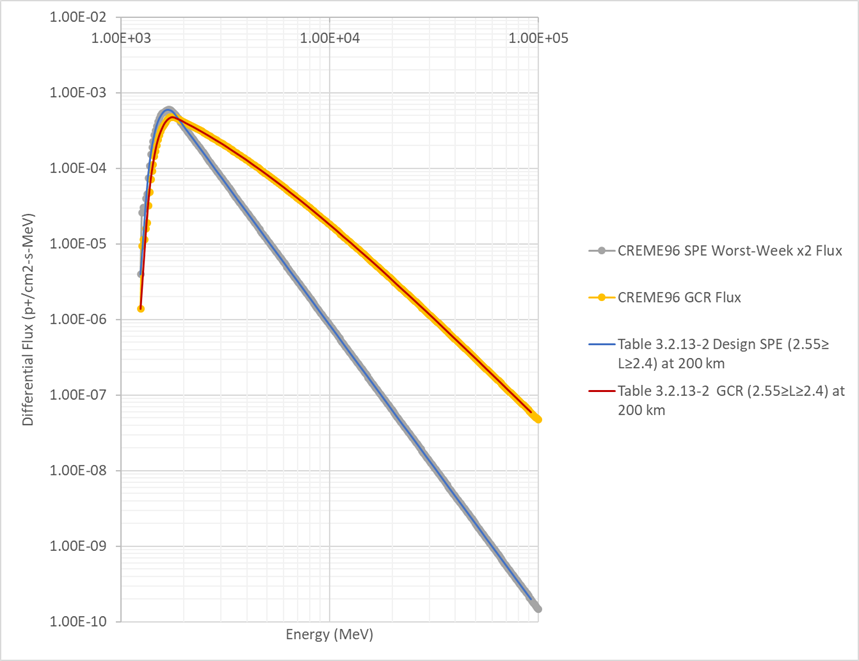
\includegraphics[width=0.95\textwidth]{DSNE_Differential_Flux_Comparison.png}
	\caption{Output generated from CREME96 \textsf{FLUX} are plotted against DSNE Table 3.2.13-2 for SPEs and GCRs.}\label{fig:DSNE_Differential_Flux_Comparison}
\end{figure}

\clearpage % forces the figure to drop before this point

\subsection{Integral Flux}

The integral flux for both the SPEs and GRCs are derived from the differential flux output. Since the flux spectra have power-law-like features, the best way to approximate the differential flux is to interpolate using a power-law fit between data points ($x_i, y_i$), i.e.
\begin{equation}\label{eq:power_law_fit}
	y(x) = y_i\left(\frac{x}{x_i}\right)^{b_i}, \text{ for $x_i \le x \le x_{i+1}$},
\end{equation}
where
\begin{equation}
	b_i = \frac{\log(y_{i+1}/y_i)}{\log(x_{i+1}/x_i)}.
\end{equation}

The integral flux ($>x$) can then be computed by integrating from some $x$ to infinity
\begin{equation}
	Y(>x) = \int_{x}^{\infty}dx'y(x').
\end{equation}
Inserting Equation \eqref{eq:power_law_fit} for $y(x)$, the integral flux becomes
\begin{equation}\label{eq:power-law_fitted_Integral_Flux}
	Y(>x_n) = \sum_{i=n}^{N-1} \frac{y_i x_i}{b_i + 1}\left[\left(\frac{x_{i+1}}{x_i}\right)^{b_i + 1} - 1\right].
\end{equation}

Applying Equation \eqref{eq:power-law_fitted_Integral_Flux} to the differential fluxes shown in Section \ref{ssec:DifferentialFlux}, the integral fluxes are derived and compared with DSNE Table 3.2.13-3 in Figure \ref{fig:DSNE_Integral_Flux_Comparison}. The comparison again shows perfect agreement and also give merit to the power-law interpolation method outlined above.

\begin{figure}[htbp!]
	\centering
	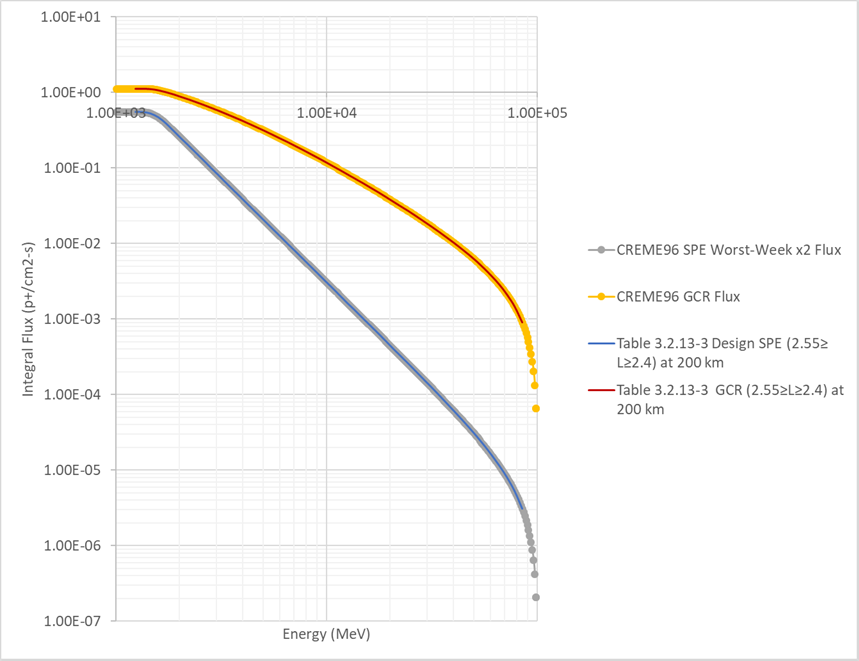
\includegraphics[width=0.95\textwidth]{DSNE_Integral_Flux_Comparison.png}
	\caption{Output generated from CREME96 \textsf{FLUX} and converted to integral fluxes using Equation \eqref{eq:power-law_fitted_Integral_Flux} are plotted against DSNE Table 3.2.13-3 for SPEs and GCRs.}\label{fig:DSNE_Integral_Flux_Comparison}
\end{figure}



\clearpage % forces the figure to drop before this point

%%%%%%%%%%%%%%%%%%%%%%%%%%%%%%%%%%%%%%%%%%%%%%%%%%%%%%%%%%%%%%%%%%
%%%%%%%%%%%%%%%%%%%%%%%%%%%%%%%%%%%%%%%%%%%%%%%%%%%%%%%%%%%%%%%%%%

\section{Updated 50 km Environment}

In this section, the methods used to derive the DSNE tables for the 200 km environments will be used to compute the new 50 km environments. The assumptions that went into the parameters used for the 50 km environments are discussed in Section~\ref{ssec:Assumptions}. Following in Section~\ref{sec:ComparisonOf50kmAnd200kmEnvironments}, the integral LET spectra, differential fluxes, and integral fluxes generated for the 50 km environments are compared to the DSNE 200 km environments.


\subsection{Assumptions}\label{ssec:Assumptions}

Information about the 3-DOF DAC-1 BOLE separation was given by Patrick Montgomery on 2/2/2021. The trajectory was optimized to produce maximum loads, so a lower separation altitude is achieved. There also was no dispersion in launch azimuth. The specific data provided is as follows:
\subsubsection{BOLE Separation Location}
\begin{itemize}
	\item Altitude (ft): $1.47769768\times 10^5$ to $1.56331111\times 10^5$ (or $45.04$ km to $47.65$ km)
	\item Geodetic Latitude (deg): $28.63679$ to $28.63769$
	\item Longitude (deg): $279.844269$ to $279.892322$
	\item Inclination (deg): $28.48989$ to $28.49106$
\end{itemize}


\subsubsection{LC-39b Location}
In order to include dispersion in launch azimuth, the downrange distance is computed assuming a launch location from KSC launch complex 39b.
\begin{itemize}
	\item Geodetic Latitude (deg): $28.627623$
	\item Longitude (deg): $279.378890$.
\end{itemize}

\subsubsection{Downrange Distance and Initial Bearing}
Given the latitude and longitude ($\phi$, $\lambda$) of the starting and ending location, a downrange distance can be computed\footnote{E.g., see \url{https://www.movable-type.co.uk/scripts/latlong.html}} using
\begin{equation}
	D = 2r_E\arcsin(\sqrt{a}),
\end{equation}
where $r_E = 6371$ km (Earth's radius), and
\begin{equation}
	a = \sin^2(\Delta\phi/2) + \cos\phi_1\cos\phi_2\sin^2(\Delta\lambda/2),
\end{equation}
for $\Delta\phi = \phi_1-\phi_2$ and $\Delta\lambda = \lambda_1-\lambda_2$.

The initial bearing from the launch point can also be calculated using
\begin{equation}\label{eq:initial-bearing-shortdist}
	\tan\theta_{i(1,2)} = \frac{\sin\Delta\lambda\cos\phi_2}{\cos\phi_1\sin\phi_2-\sin\phi_1\cos\phi_2\cos\Delta\lambda}.
\end{equation}

Therefore, from the initial separation data, the bearing and downrange distance is the following:
\begin{itemize}
	\item \textbf{Nominal bearing} (deg, from N CCW): $-88.48$ to $-88.71$ (i.e., almost strictly due East)
	\item \textbf{Downrange distance} (km): $45.4$ to $50.1$.
\end{itemize}

The range of valid bearings from KSC LC-39b are $-35^\circ$ to $-120^\circ$, where the worst-case\footnote{Worst-case in terms of a larger L-shell value, giving less magnetic field protection from space radiation.} would be $-35^\circ$ (most northerly direction), giving an orbital inclination of $57^\circ$.

\subsubsection{Magnetic Epoch and L-Shell}\label{sssec:MagneticEpochAndL-Shell}
A magnetic epoch must be selected in order to convert geodetic latitude and longitude to magnetic latitude and longitude. The magnetic latitude and separation altitude are used to compute the L-shell. In DSNE, it is implicitly assumed that the magnetic epoch is 1980, driven by the assumptions built into CREME96. However, a magnetic epoch of 2020 is also used in the analysis for the lower bound\footnote{Currently, the magnetic south pole (near the geographic north pole) has been migrating towards the Asian continent, hence putting KSC at a lower L-shell over several decades.} on the L-shell.

The L-shell can be computed by
\begin{equation}
	L = \frac{1 + \frac{h}{R_E}}{\cos(\phi_{\text{geomagnetic}})},
\end{equation}
were $h$ is the spacecraft altitude, $R_E = 6371$ km, and $\phi_{\text{geomagnetic}}$ is the geomagnetic latitude.

If a most-northerly(southerly) launch azimuth case is assumed, the magnetic latitude for different magnetic epochs is given in Table \ref{tab:magnetic_lat_ranges}.
\begin{table}[h]\centering
	\caption{The magnetic latitudes at BOLE separation for magnetic epochs of 1980 \& 2020 and bounding cases for launch azimuths ($65^\circ$ to $-30^\circ$).}\label{tab:magnetic_lat_ranges}
	\begin{tabular}{|c | c | c |}\hline
		 & 1980 epoch & 2020 epoch  \\\hline
		Most-northerly & $39.83^\circ$ & $38.14^\circ$ \\\hline
		Most-southerly & $39.23^\circ$ & $37.54^\circ$ \\\hline
	\end{tabular}
\end{table}

\paragraph{L-Shell Sensitivity:}
The L-shell sensitivity, or $dL$, is affected by magnetic epoch, launch azimuth, and separation altitude, summarized below:
\begin{itemize}
	\item Magnetic epoch: Magnetic latitude difference of $1.69^\circ$ ($dL \approx 0.08$ or $72\%$ of total $dL$)
	\item Launch azimuth: Magnetic latitude difference of $0.60^\circ$ ($dL \approx 0.03$ or $27\%$ of total $dL$)
	\item Altitude at separation: Altitude difference of $5$ km ($dL \approx 0.0013$ or $1\%$ of total $dL$)
\end{itemize}
Therefore, the choice of magnetic epoch drives the range of the L-shell compared to the launch azimuth range and range in separation altitude.

\subsubsection{L-Shell Range}
Given the analysis in Section \ref{sssec:MagneticEpochAndL-Shell}, the L-shell range used in deriving the new 50 km environments is:
\begin{itemize}
	\item From $1.60174$ (most southerly launch azimuth, 2020 magnetic epoch, and separation altitude of 45 km)
	\item To $1.70896$ (most northerly launch azimuth, 1980 magnetic epoch, and separation altitude of 50 km).
\end{itemize}

The difference from using a separation altitude of 47.65 km vs.\ 50 km changes the L-shell value only in the last two significant figures.

\subsection{\textsf{GTRN}, \textsf{FLUX}, and \textsf{LETSPEC} Options for 50 km Environments}
The options used in the \textsf{GTRN} routine for the 50 km environments (as a best guess worst-case) are as follows:

\begin{itemize}
	\item 1.C.a. \& 1.C.b. 50 km circular orbit
	\item 1.C.c. 57 degrees orbit inclination
	\item 1.C.g. Effective L-shell range: $1.60174 \le L \le 1.70896$
	\item 2. Stormy magnetic weather conditions.
\end{itemize}

Options for the \textsf{FLUX} and \textsf{LETSPEC} routines are the same as in Sections \ref{ssec:DifferentialFlux} and \ref{ssec:LET}, respectively.

%%%%%%%%%%%%%%%%%%%%%%%%%%%%%%%%%%%%%%%%%%%%%%%%%%%%%%%%%%%%%%%%%%
%%%%%%%%%%%%%%%%%%%%%%%%%%%%%%%%%%%%%%%%%%%%%%%%%%%%%%%%%%%%%%%%%%

\section{Comparison of 50 km and 200 km Environments}\label{sec:ComparisonOf50kmAnd200kmEnvironments}

\subsection{Linear Energy Transfer (LET)}

The high resolution tables for the SPE and GCR LET spectra are given in Appendix~\ref{asec:ProcessCREME96Data}, Listings \ref{lst:SPE_LET_worst-case} and \ref{lst:GCR_LET_worst-case}. For a lower resolution table (that would conform to what is in DSNE), see Table \ref{tab:50kmIntegralLET}.

\begin{figure}[htbp!]
	\centering
	\begin{subfigure}[b]{0.65\textwidth}
		\centering
		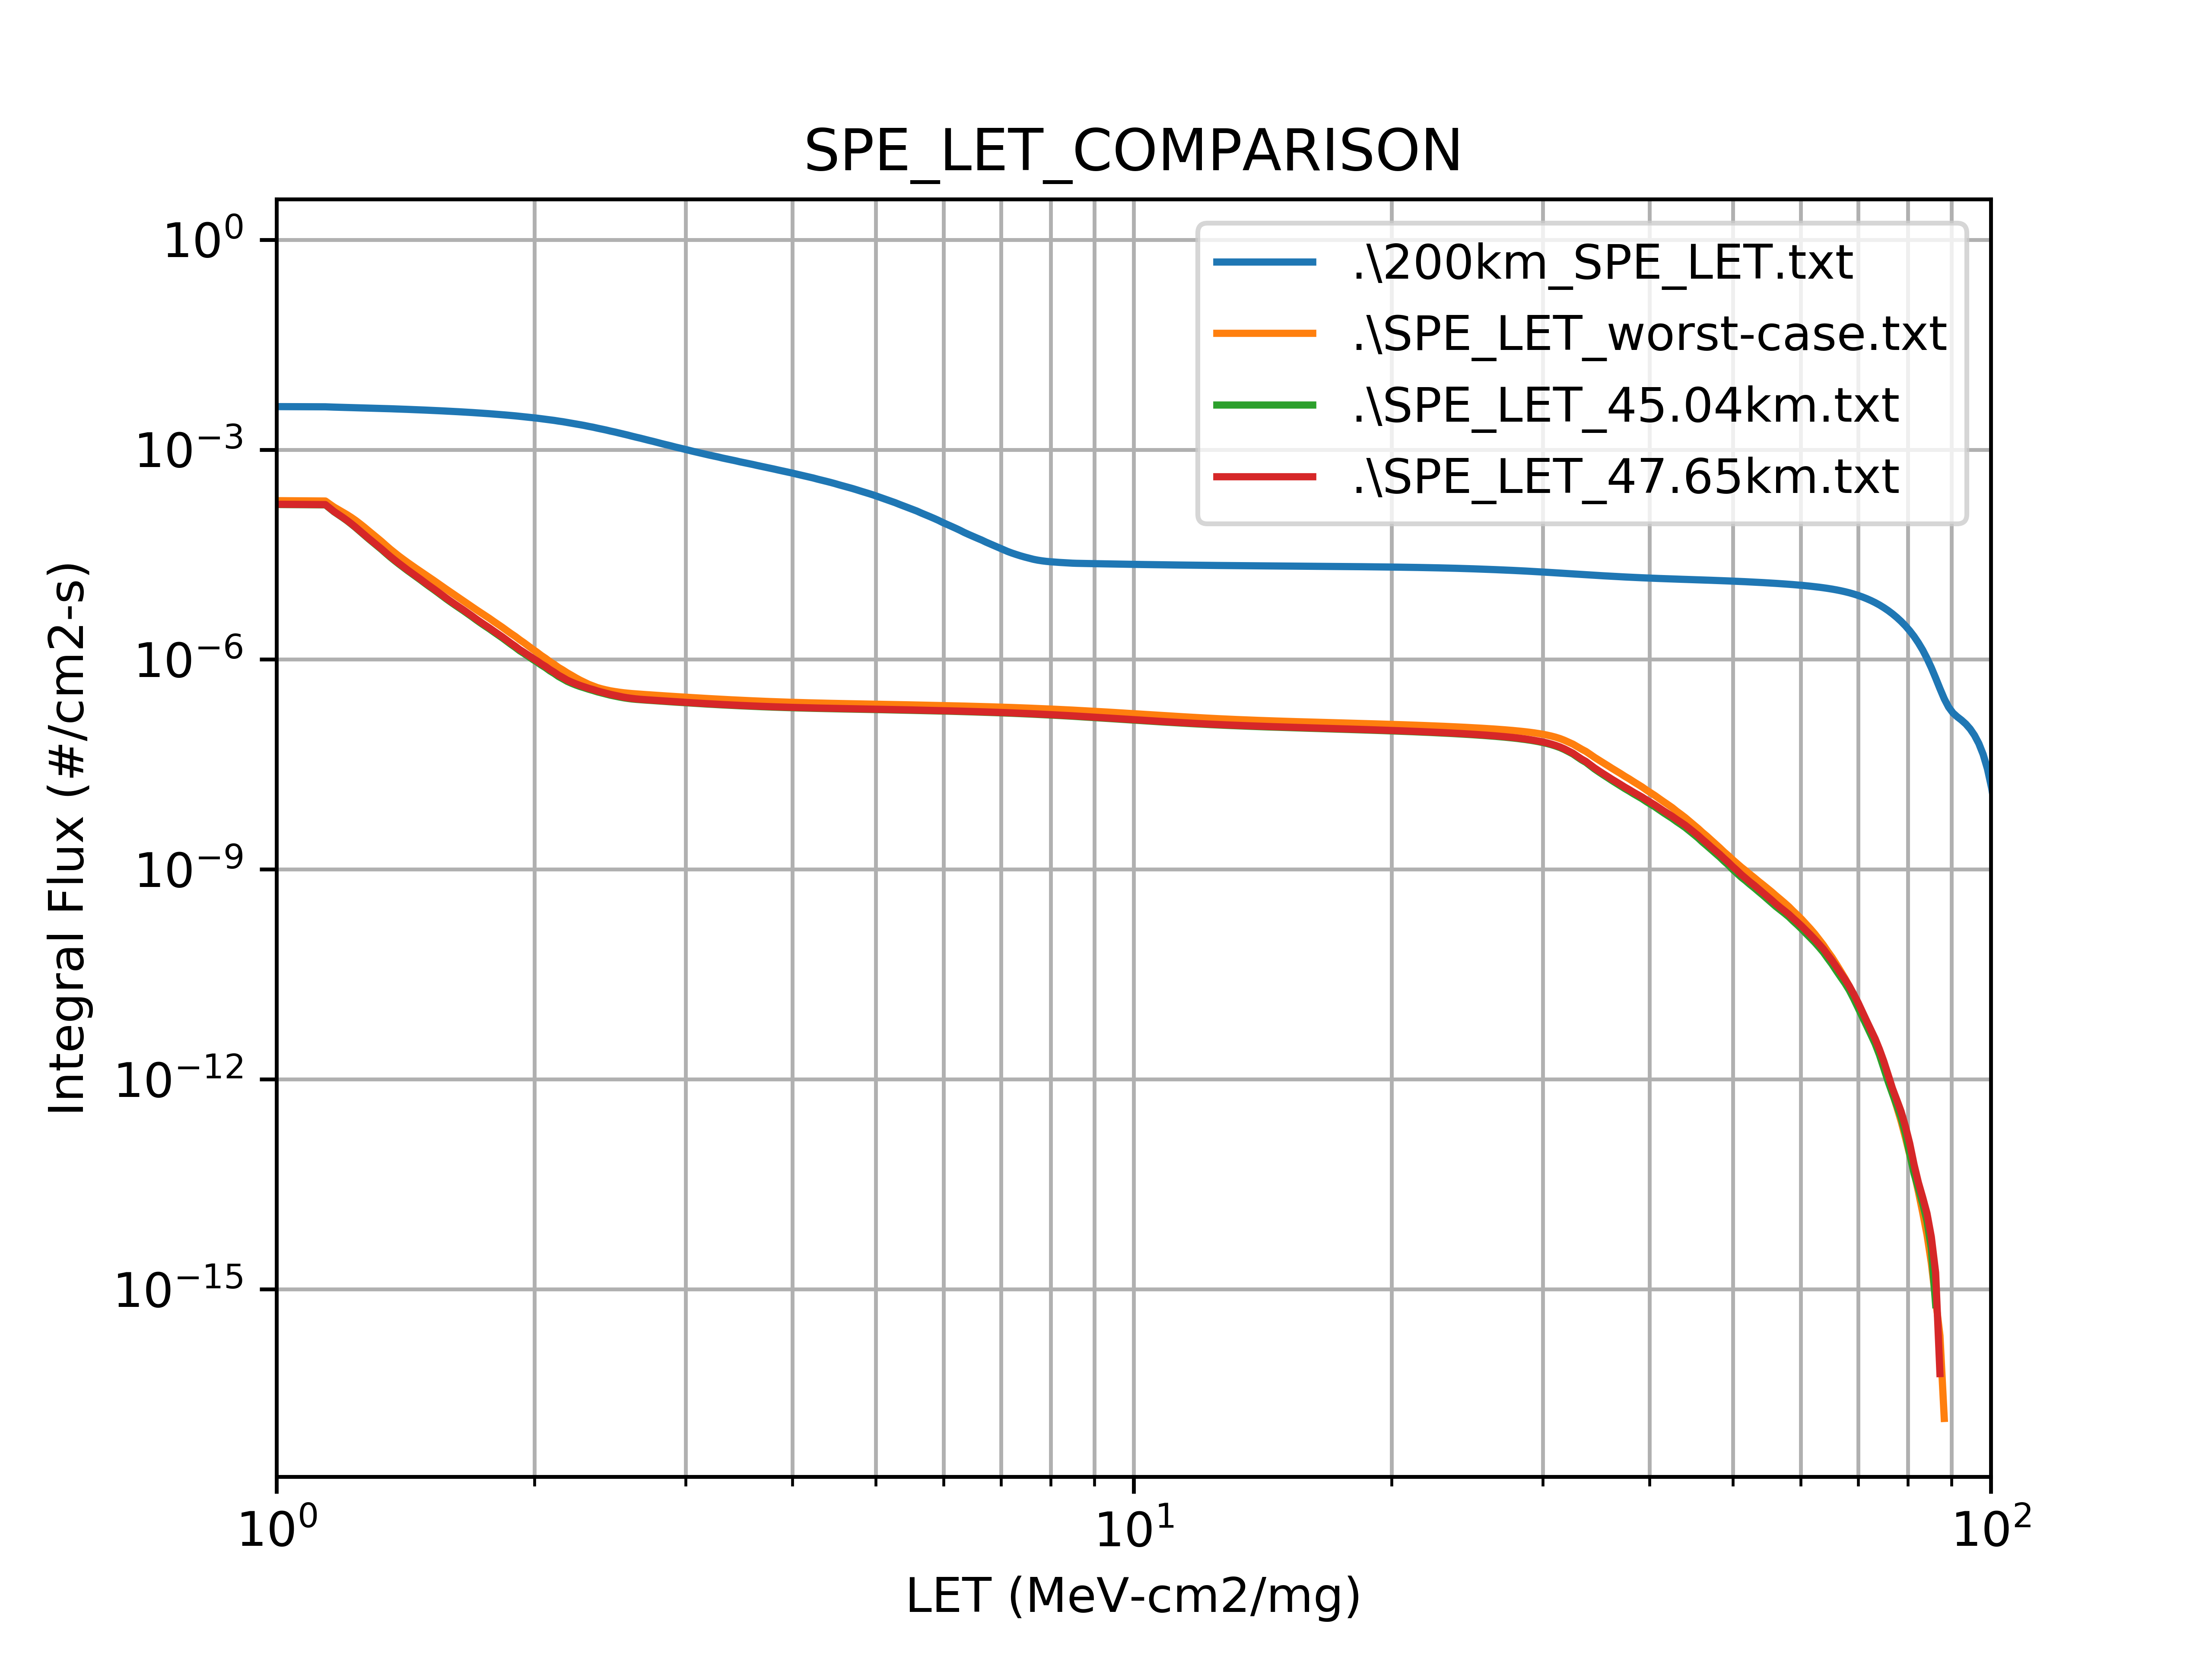
\includegraphics[width=\textwidth]{SPE_LET_COMPARISON.png}
		\caption{Comparing different SPE LET BOLE environments with 200 km DSNE environment.}
		\label{sfig:SPE_LET_COMPARISON}
	\end{subfigure}
	\hfill
	\begin{subfigure}[b]{0.65\textwidth}
		\centering
		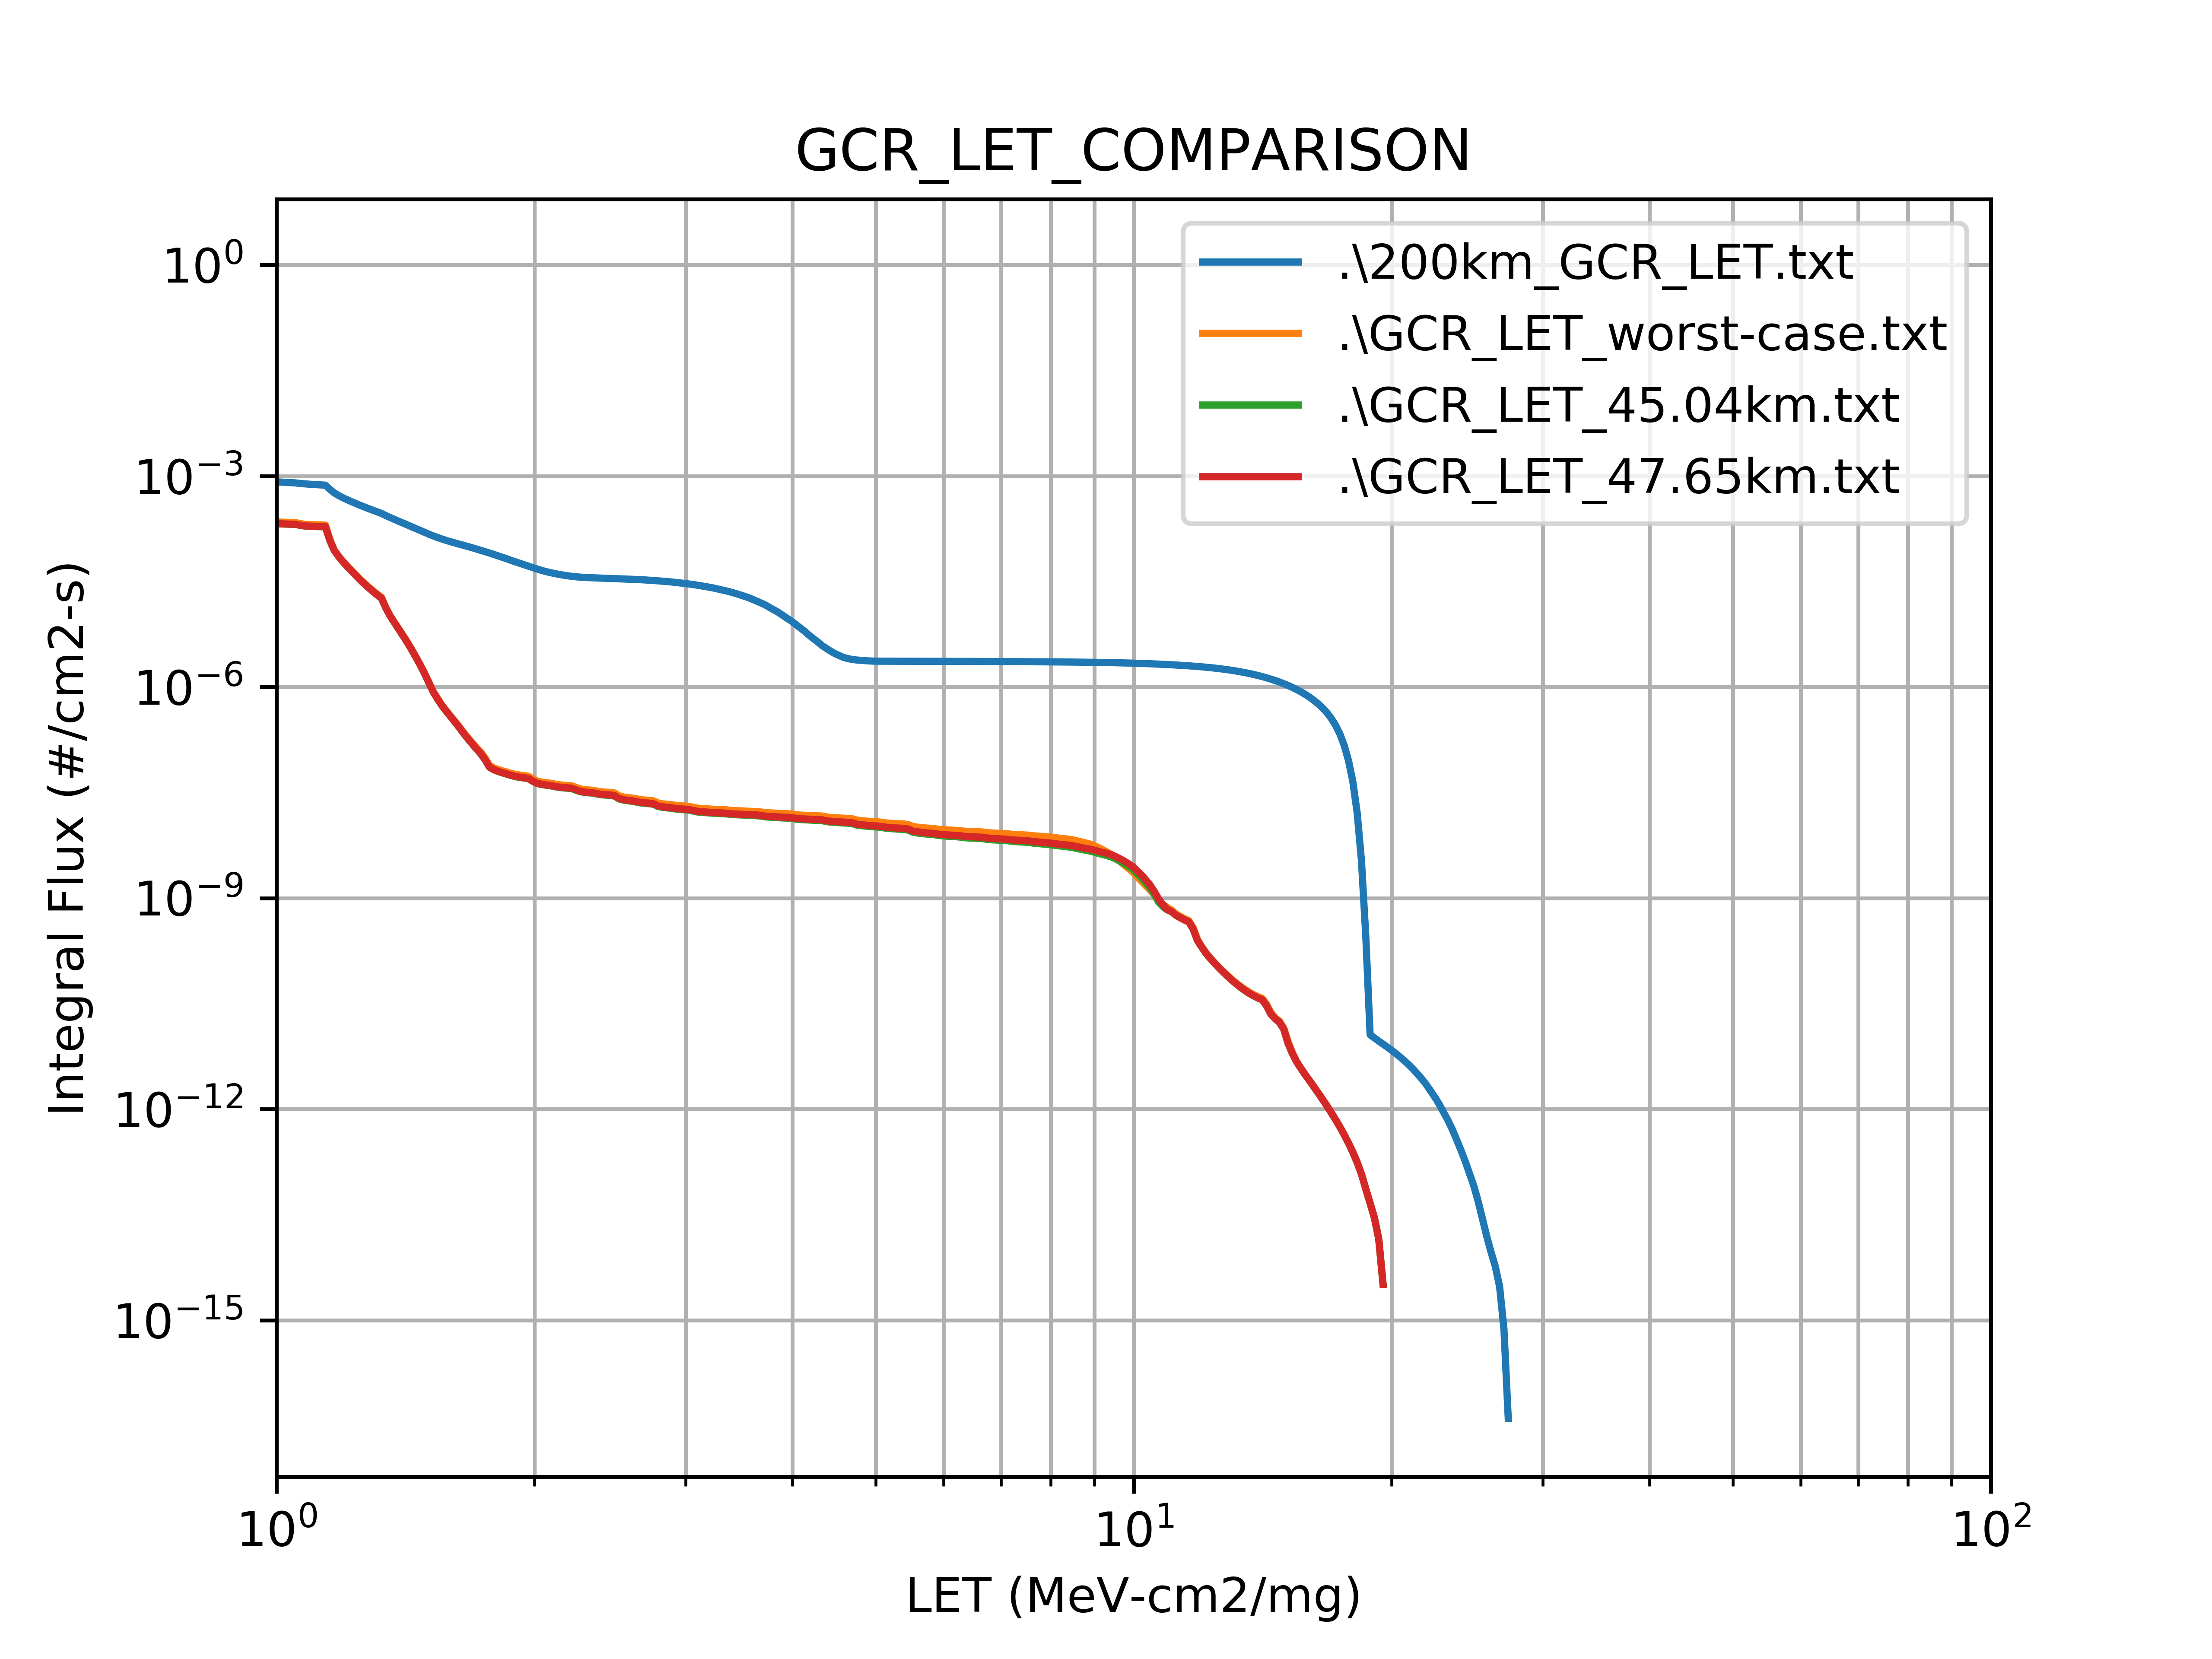
\includegraphics[width=\textwidth]{GCR_LET_COMPARISON.png}
		\caption{Comparing different GCR LET BOLE environments with 200 km DSNE environment.}
		\label{sfig:GCR_LET_COMPARISON}
	\end{subfigure}
	\caption{Comparison of integral LET fluxes between 50 km and 200 km environments.}
	\label{fig:LET_COMPARISON}
\end{figure}

\begin{table}[h]
	\caption{50 km Integral LET Flux as Shown in Figure \ref{fig:LET_COMPARISON}, worst-case lines.}
	\label{tab:50kmIntegralLET}\centering
	\resizebox{0.65\textwidth}{!}{%
		\begin{tabular}{|c|c|c|}
			\hline
			\rowcolor{DSNE-Blue} &\textbf{Design SPE} & \textbf{GCR} \\ \hline
			\rowcolor{DSNE-Gray} \textbf{LET (MeV-cm$^2$/mg)} & \textbf{Integral Flux (\#/cm$^2$-s)} & \textbf{Integral Flux (\#/cm$^2$-s)} \\ \hline
			1.00E+00&	1.86E-04&	2.23E-04 \\ \hline
			1.10E+00&	1.84E-04&	2.04E-04\\ \hline
			1.20E+00&	1.24E-04&	5.81E-05\\ \hline
			1.31E+00&	5.31E-05&	2.04E-05\\ \hline
			1.44E+00&	2.19E-05&	3.32E-06\\ \hline
			1.58E+00&	1.01E-05&	4.63E-07\\ \hline
			1.73E+00&	4.73E-06&	1.21E-07\\ \hline
			1.89E+00&	2.19E-06&	5.80E-08\\ \hline
			2.07E+00&	9.77E-07&	4.33E-08\\ \hline
			2.27E+00&	4.92E-07&	3.53E-08\\ \hline
			2.49E+00&	3.46E-07&	3.04E-08\\ \hline
			2.73E+00&	3.11E-07&	2.44E-08\\ \hline
			2.99E+00&	2.90E-07&	2.03E-08\\ \hline
			3.27E+00&	2.71E-07&	1.82E-08\\ \hline
			3.58E+00&	2.56E-07&	1.71E-08\\ \hline
			3.92E+00&	2.45E-07&	1.58E-08\\ \hline
			4.30E+00&	2.38E-07&	1.47E-08\\ \hline
			4.71E+00&	2.32E-07&	1.33E-08\\ \hline
			5.16E+00&	2.27E-07&	1.16E-08\\ \hline
			5.65E+00&	2.22E-07&	1.00E-08\\ \hline
			6.19E+00&	2.17E-07&	9.19E-09\\ \hline
			6.78E+00&	2.10E-07&	8.47E-09\\ \hline
			7.43E+00&	2.03E-07&	7.90E-09\\ \hline
			8.14E+00&	1.93E-07&	7.17E-09\\ \hline
			8.91E+00&	1.82E-07&	5.79E-09\\ \hline
			9.76E+00&	1.71E-07&	2.92E-09\\ \hline
			1.07E+01&	1.59E-07&	9.12E-10\\ \hline
			1.17E+01&	1.49E-07&	3.93E-10\\ \hline
			1.28E+01&	1.40E-07&	8.18E-11\\ \hline
			1.41E+01&	1.34E-07&	3.83E-11\\ \hline
			1.54E+01&	1.29E-07&	5.54E-12\\ \hline
			1.69E+01&	1.25E-07&	1.04E-12\\ \hline
			1.85E+01&	1.21E-07&	1.10E-13\\ \hline
			2.02E+01&	1.17E-07&	0.00E+00\\ \hline
			2.22E+01&	1.13E-07&	0.00E+00\\ \hline
			2.43E+01&	1.07E-07&	0.00E+00\\ \hline
			2.66E+01&	1.00E-07&	0.00E+00\\ \hline
			2.91E+01&	9.00E-08&	0.00E+00\\ \hline
			3.19E+01&	6.84E-08&	0.00E+00\\ \hline
			3.50E+01&	3.58E-08&	0.00E+00\\ \hline
			3.83E+01&	1.79E-08&	0.00E+00\\ \hline
			4.20E+01&	8.48E-09&	0.00E+00\\ \hline
			4.60E+01&	3.46E-09&	0.00E+00\\ \hline
			5.04E+01&	1.27E-09&	0.00E+00\\ \hline
			5.52E+01&	5.07E-10&	0.00E+00\\ \hline
			6.04E+01&	1.82E-10&	0.00E+00\\ \hline
			6.62E+01&	4.21E-11&	0.00E+00\\ \hline
			7.25E+01&	4.54E-12&	0.00E+00\\ \hline
			7.94E+01&	1.54E-13&	0.00E+00\\ \hline
			8.70E+01&	2.84E-16&	0.00E+00\\ \hline	
		\end{tabular}%
	}
\end{table}

\clearpage % forces the figure to drop before this point



\subsection{Differential Flux}

High resolution tables shown in Appendix \ref{asec:ProcessCREME96Data} in Listings \ref{lst:SPE_flux_worst-case} and \ref{lst:GCR_flux_worst-case}. The low resolution data is shown in Table \ref{tab:50kmDifferentialFlux}.

\begin{figure}[htbp!]
	\centering
	\begin{subfigure}[b]{0.65\textwidth}
		\centering
		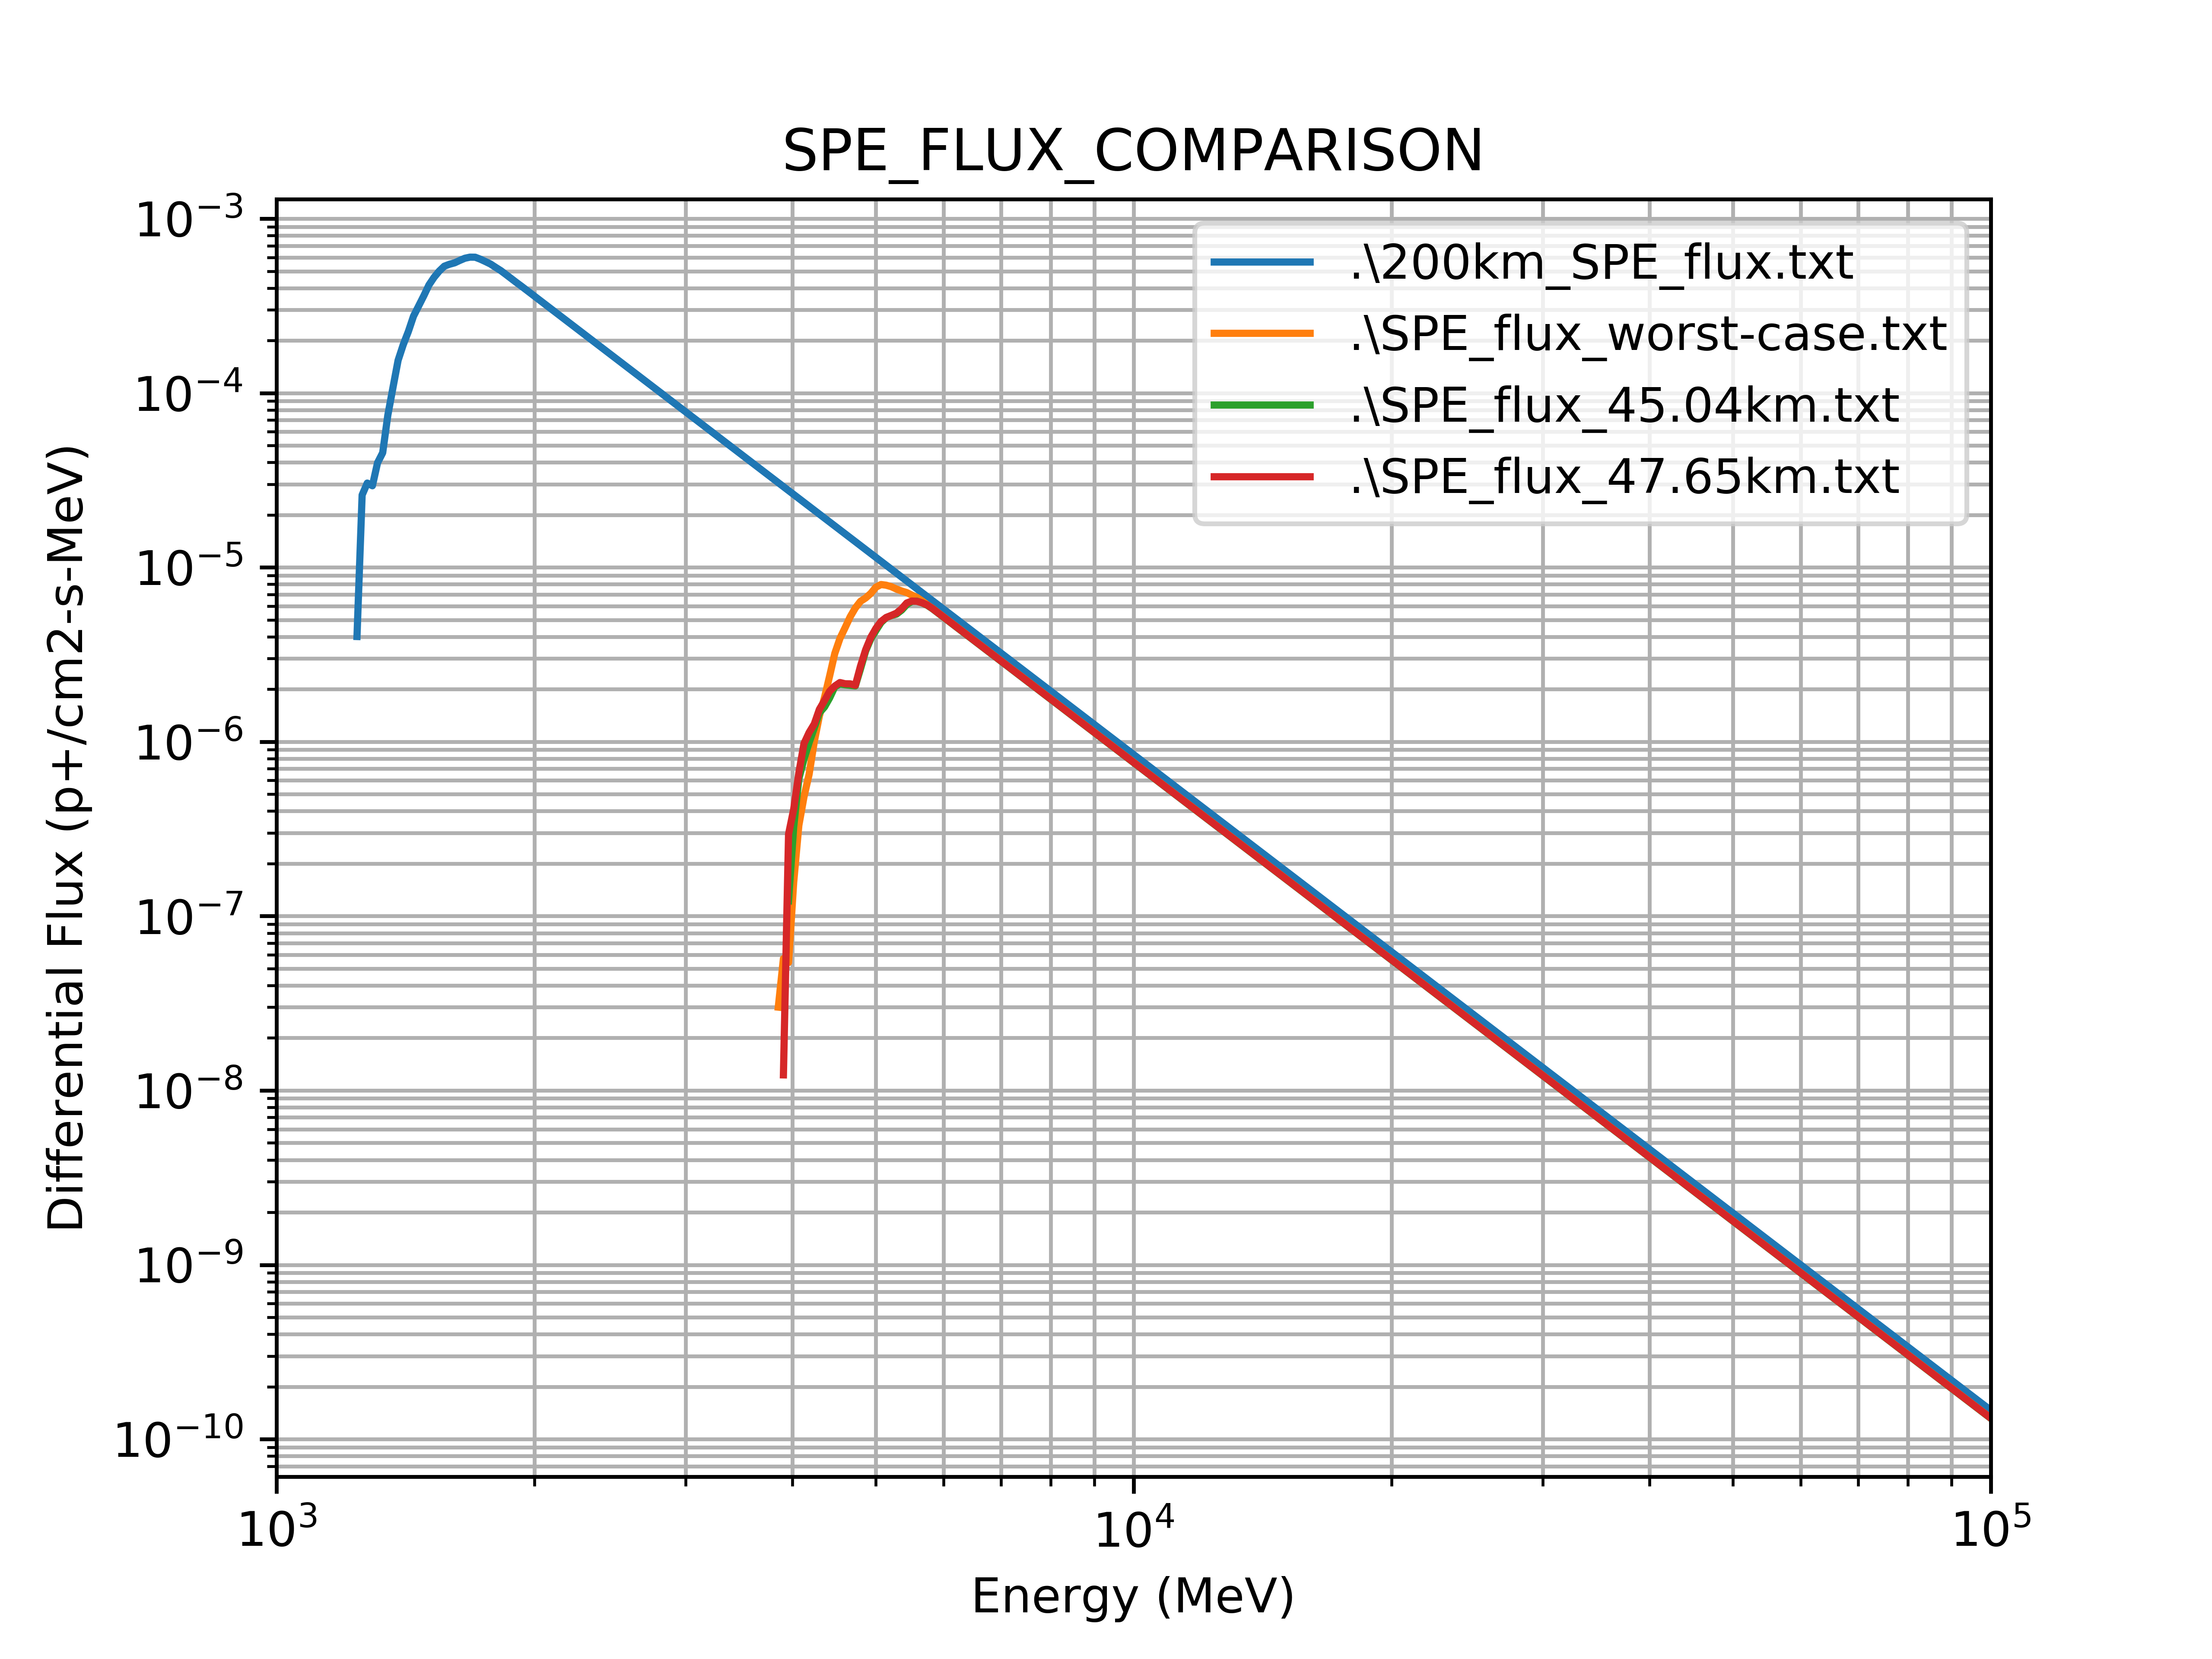
\includegraphics[width=\textwidth]{SPE_FLUX_COMPARISON.png}
		\caption{Comparing different differential SPE flux BOLE environments with 200~km DSNE environment.}
		\label{sfig:SPE_FLUX_COMPARISON}
	\end{subfigure}
	\hfill
	\begin{subfigure}[b]{0.65\textwidth}
		\centering
		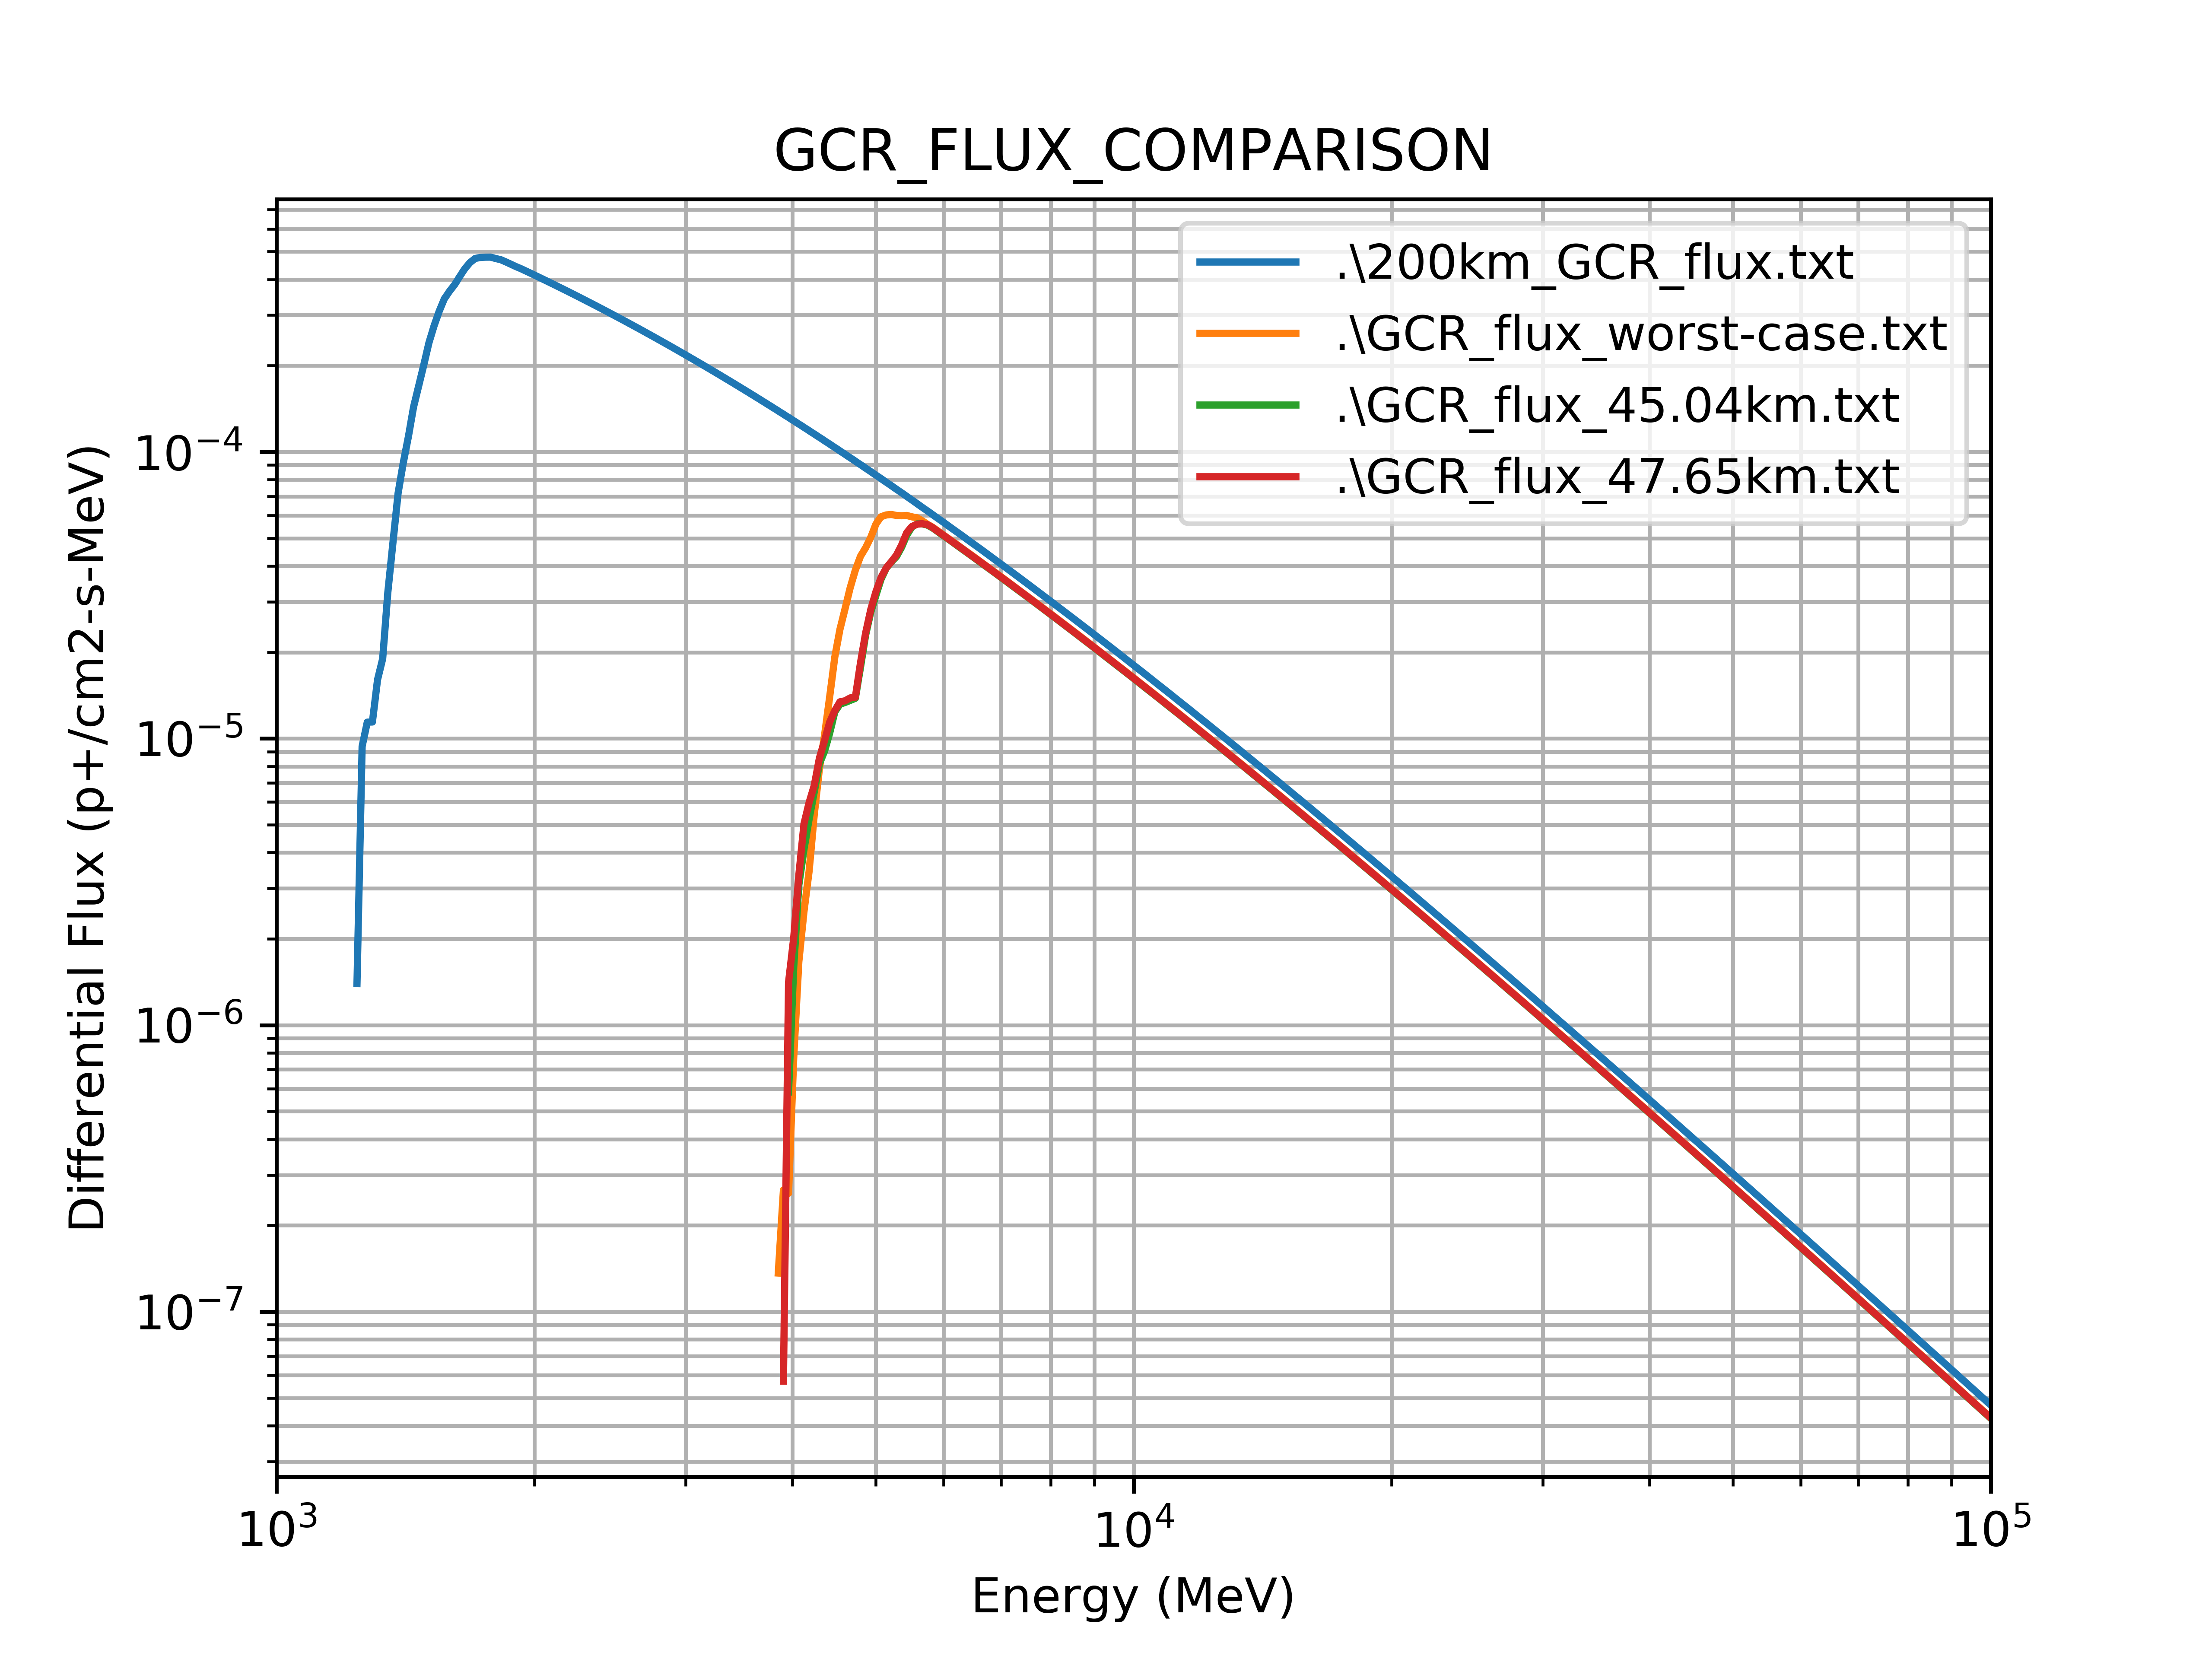
\includegraphics[width=\textwidth]{GCR_FLUX_COMPARISON.png}
		\caption{Comparing different differential GCR flux BOLE environments with 200~km DSNE environment.}
		\label{sfig:GCR_FLUX_COMPARISON}
	\end{subfigure}
	\caption{Comparison of differential fluxes between 50 km and 200 km environments.}
	\label{fig:FLUX_COMPARISON}
\end{figure}


\begin{table}[h]
	\caption{50 km Differential Flux as Shown in Figure \ref{fig:FLUX_COMPARISON}, worst-case lines.}
	\label{tab:50kmDifferentialFlux}\centering
	\resizebox{0.65\textwidth}{!}{%
		\begin{tabular}{|c|c|c|}
			\hline
			\rowcolor{DSNE-Blue} &\textbf{Design SPE} & \textbf{GCR} \\ \hline
			\rowcolor{DSNE-Gray} \textbf{Energy (MeV)} & \textbf{Differential Flux (p+/cm$^2$-s-MeV)} & \textbf{Differential Flux (p+/cm$^2$-s-MeV)} \\ \hline
			3.90E+03&	5.50E-08&	2.56E-07\\ \hline
			4.17E+03&	5.99E-07&	3.17E-06\\ \hline
			4.45E+03&	2.77E-06&	1.66E-05\\ \hline
			4.75E+03&	6.00E-06&	4.01E-05\\ \hline
			5.08E+03&	7.97E-06&	5.95E-05\\ \hline
			5.42E+03&	7.19E-06&	6.00E-05\\ \hline
			5.79E+03&	5.92E-06&	5.50E-05\\ \hline
			6.19E+03&	4.63E-06&	4.78E-05\\ \hline
			6.61E+03&	3.61E-06&	4.14E-05\\ \hline
			7.06E+03&	2.82E-06&	3.58E-05\\ \hline
			7.55E+03&	2.20E-06&	3.09E-05\\ \hline
			8.06E+03&	1.72E-06&	2.66E-05\\ \hline
			8.61E+03&	1.34E-06&	2.29E-05\\ \hline
			9.20E+03&	1.04E-06&	1.97E-05\\ \hline
			9.83E+03&	8.15E-07&	1.68E-05\\ \hline
			1.05E+04&	6.35E-07&	1.44E-05\\ \hline
			1.12E+04&	4.96E-07&	1.23E-05\\ \hline
			1.20E+04&	3.87E-07&	1.05E-05\\ \hline
			1.28E+04&	3.02E-07&	8.96E-06\\ \hline
			1.37E+04&	2.35E-07&	7.62E-06\\ \hline
			1.46E+04&	1.84E-07&	6.48E-06\\ \hline
			1.56E+04&	1.43E-07&	5.50E-06\\ \hline
			1.67E+04&	1.12E-07&	4.67E-06\\ \hline
			1.78E+04&	8.72E-08&	3.95E-06\\ \hline
			1.90E+04&	6.80E-08&	3.35E-06\\ \hline
			2.03E+04&	5.31E-08&	2.83E-06\\ \hline
			2.17E+04&	4.14E-08&	2.39E-06\\ \hline
			2.32E+04&	3.23E-08&	2.02E-06\\ \hline
			2.48E+04&	2.52E-08&	1.70E-06\\ \hline
			2.64E+04&	1.97E-08&	1.44E-06\\ \hline
			2.82E+04&	1.53E-08&	1.21E-06\\ \hline
			3.02E+04&	1.20E-08&	1.02E-06\\ \hline
			3.22E+04&	9.34E-09&	8.57E-07\\ \hline
			3.44E+04&	7.29E-09&	7.21E-07\\ \hline
			3.68E+04&	5.69E-09&	6.06E-07\\ \hline
			3.93E+04&	4.44E-09&	5.09E-07\\ \hline
			4.20E+04&	3.46E-09&	4.27E-07\\ \hline
			4.48E+04&	2.70E-09&	3.59E-07\\ \hline
			4.79E+04&	2.11E-09&	3.01E-07\\ \hline
			5.12E+04&	1.64E-09&	2.52E-07\\ \hline
			5.47E+04&	1.28E-09&	2.12E-07\\ \hline
			5.84E+04&	1.00E-09&	1.77E-07\\ \hline
			6.24E+04&	7.80E-10&	1.48E-07\\ \hline
			6.66E+04&	6.09E-10&	1.24E-07\\ \hline
			7.12E+04&	4.75E-10&	1.04E-07\\ \hline
			7.60E+04&	3.71E-10&	8.71E-08\\ \hline
			8.12E+04&	2.89E-10&	7.29E-08\\ \hline
			8.68E+04&	2.26E-10&	6.10E-08\\ \hline
			9.27E+04&	1.76E-10&	5.10E-08\\ \hline
			9.90E+04&	1.37E-10&	4.27E-08\\ \hline
		\end{tabular}%
	}
\end{table}


\clearpage % forces the figure to drop before this point

\subsection{Integral Flux}

High resolution tables are omitted from the appendix since they can be derived from Listings \ref{lst:SPE_flux_worst-case} and \ref{lst:GCR_flux_worst-case} by applying Equation \eqref{eq:power-law_fitted_Integral_Flux}. The low resolution data is shown in Table~\ref{tab:50kmIntegralFlux}.

\begin{figure}[htbp!]
	\centering
	\begin{subfigure}[b]{0.65\textwidth}
		\centering
		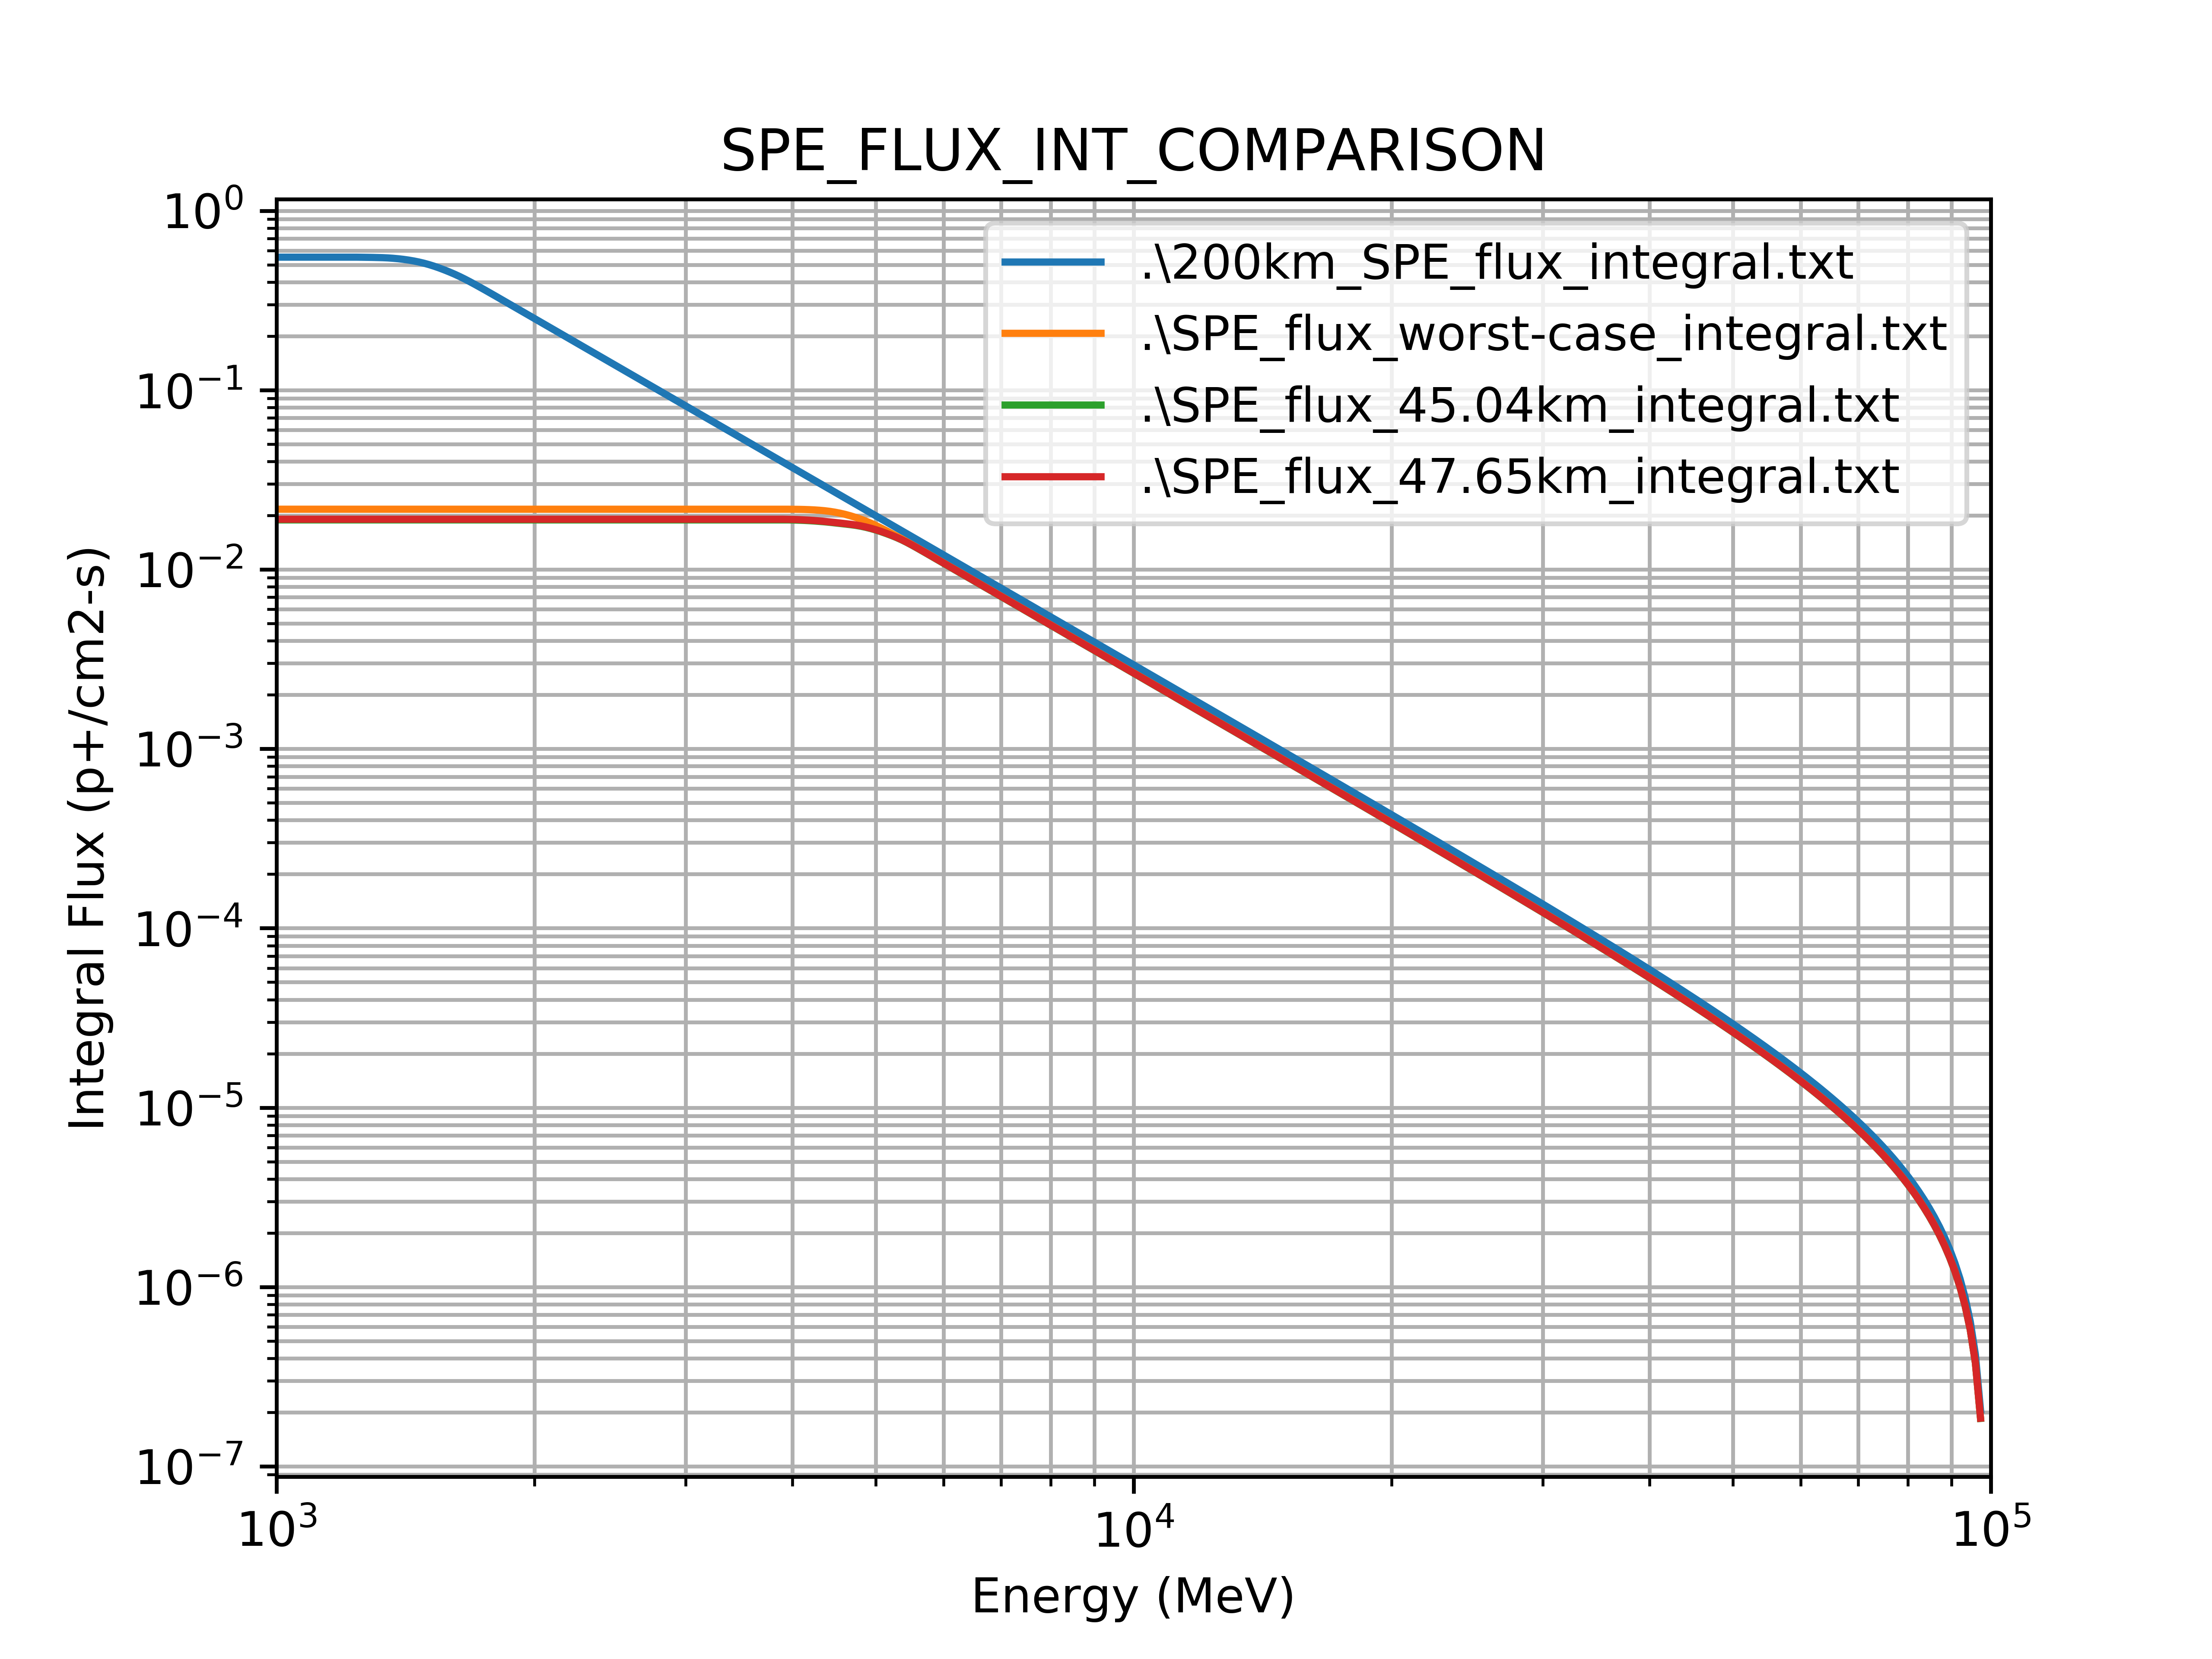
\includegraphics[width=\textwidth]{SPE_FLUX_INT_COMPARISON.png}
		\caption{Comparing different integral SPE flux BOLE environments with 200~km DSNE environment.}
		\label{sfig:SPE_FLUX_INT_COMPARISON}
	\end{subfigure}
	\hfill
	\begin{subfigure}[b]{0.65\textwidth}
		\centering
		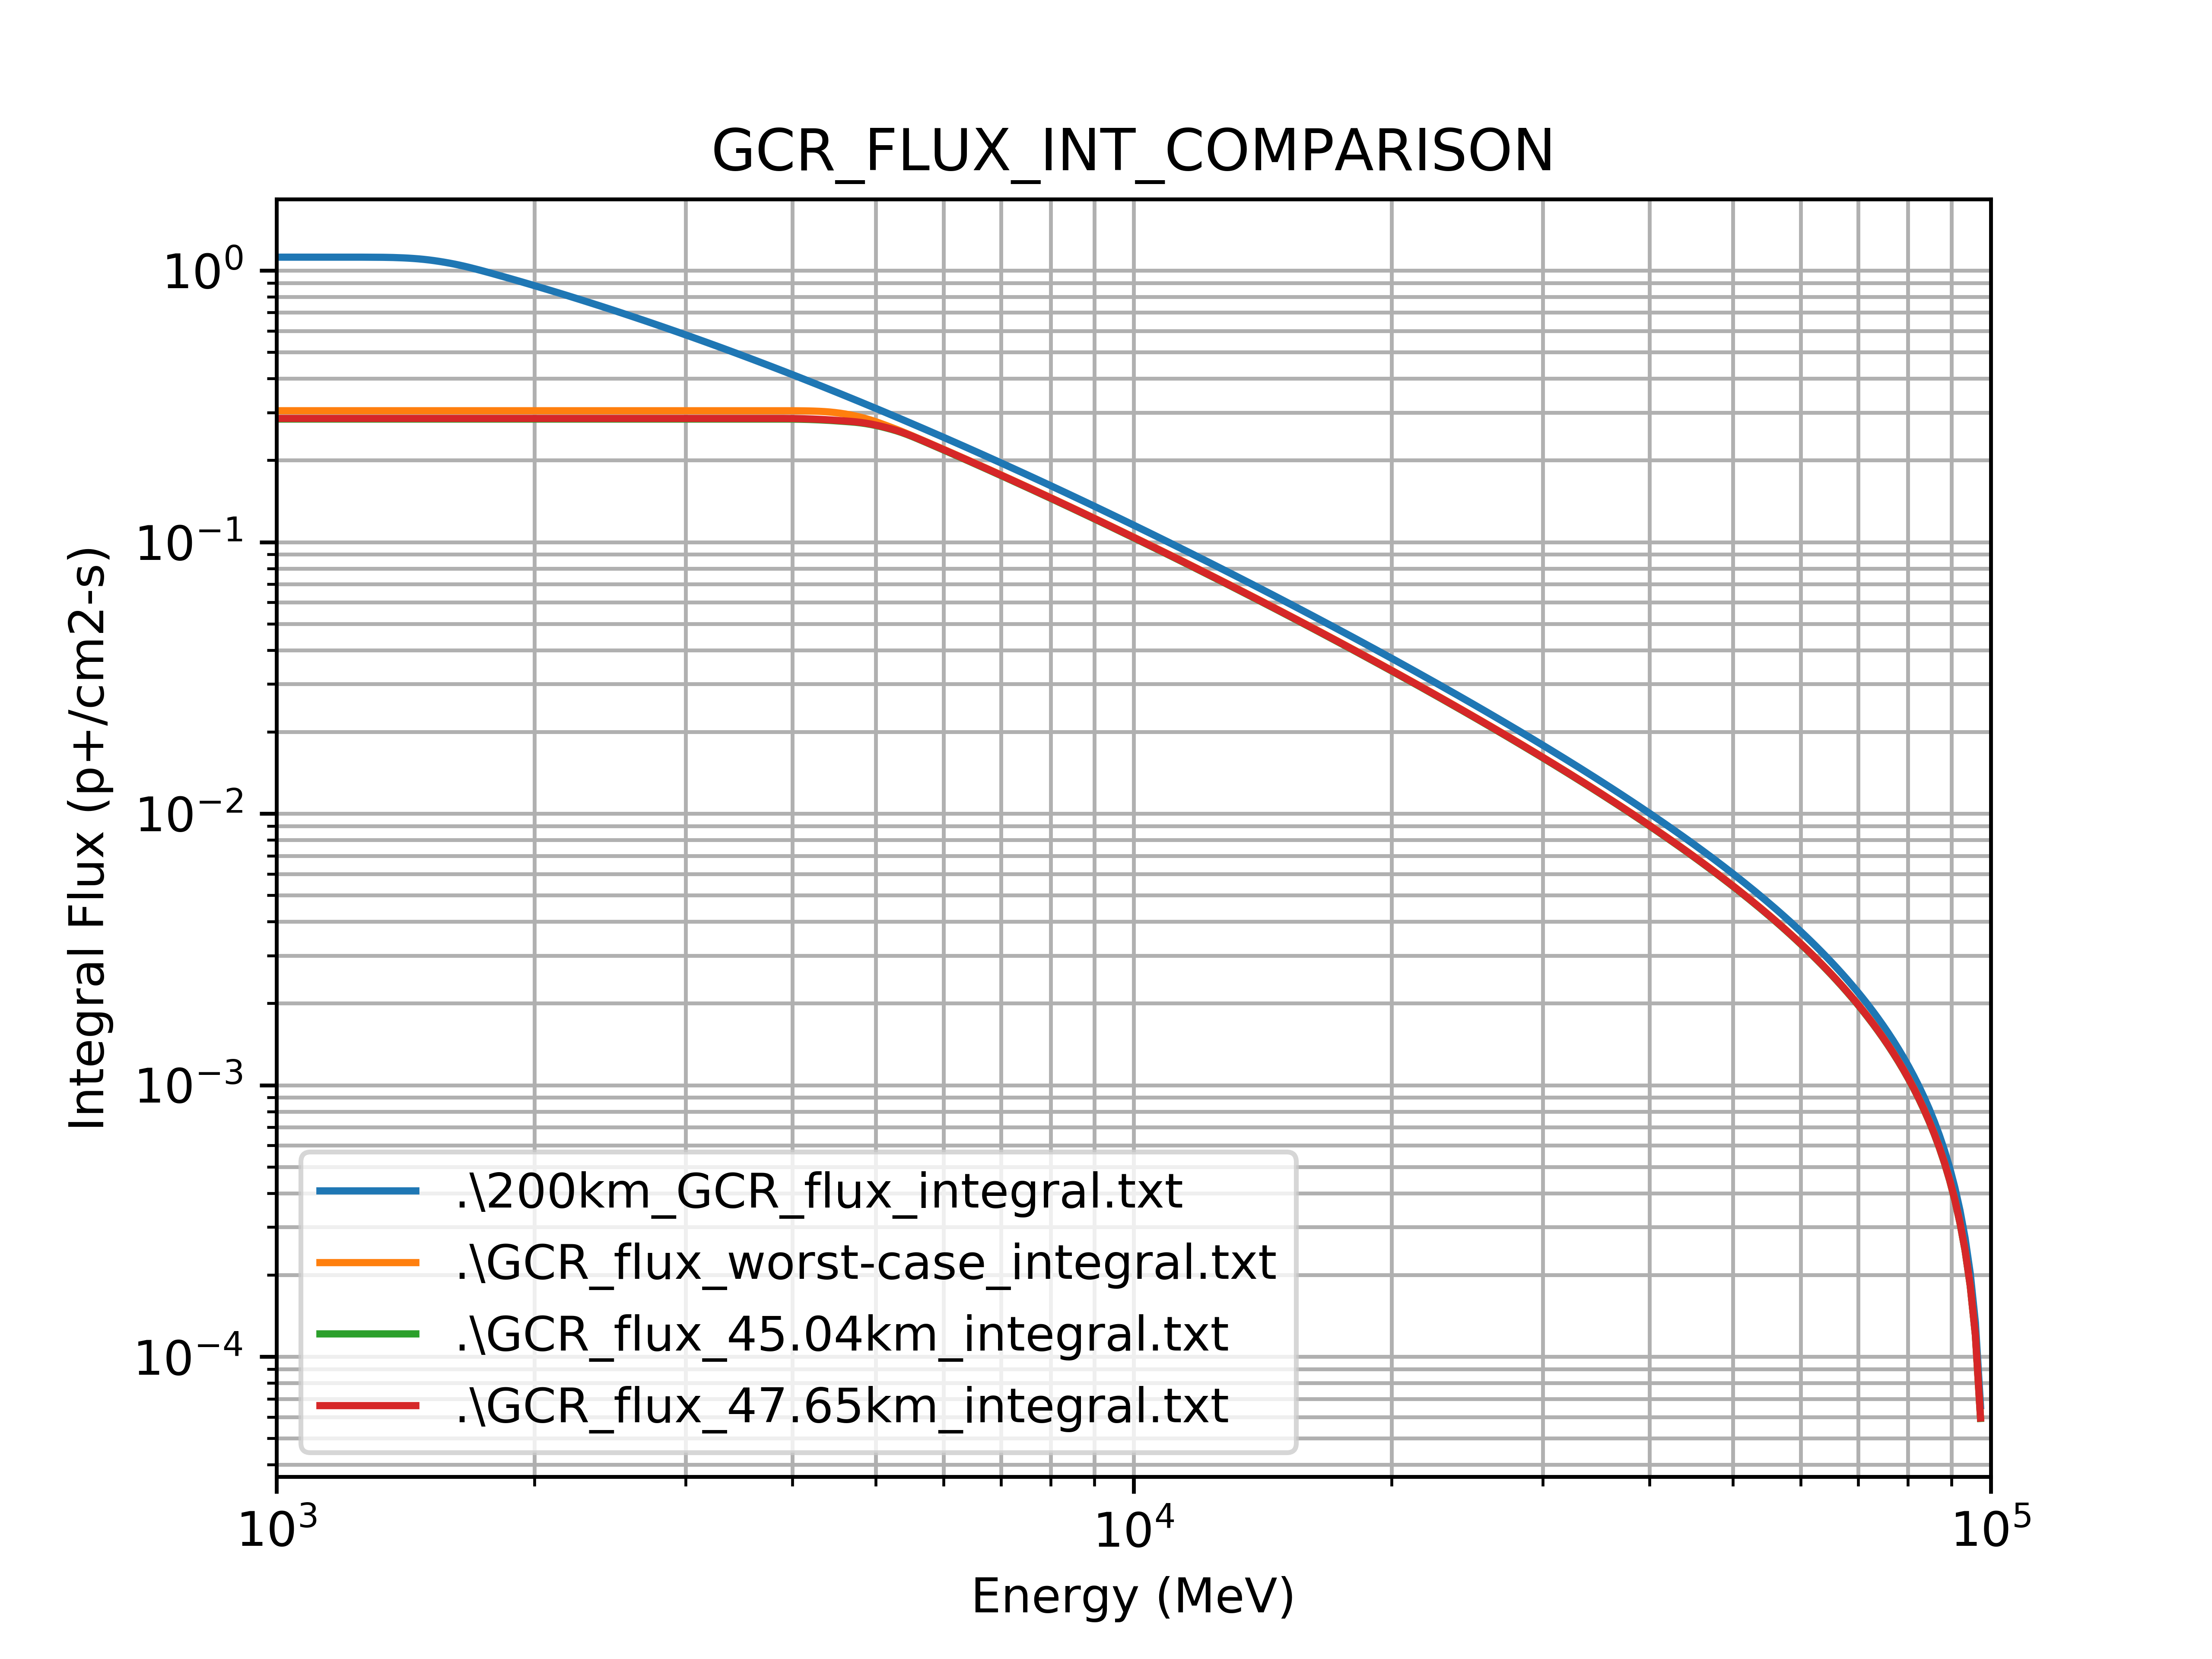
\includegraphics[width=\textwidth]{GCR_FLUX_INT_COMPARISON.png}
		\caption{Comparing different integral GCR flux BOLE environments with 200~km DSNE environment.}
		\label{sfig:GCR_FLUX_INT_COMPARISON}
	\end{subfigure}
	\caption{Comparison of integral fluxes between 50 km and 200 km environments.}
	\label{fig:FLUX_INT_COMPARISON}
\end{figure}

\begin{table}[h]
	\caption{50 km Integral Flux as Shown in Figure \ref{fig:FLUX_INT_COMPARISON}, worst-case lines.}
	\label{tab:50kmIntegralFlux}\centering
	\resizebox{0.65\textwidth}{!}{%
		\begin{tabular}{|c|c|c|}
			\hline
			\rowcolor{DSNE-Blue} &\textbf{Design SPE} & \textbf{GCR} \\ \hline
			\rowcolor{DSNE-Gray} \textbf{Energy (MeV)} & \textbf{Integral Flux (p+/cm$^2$-s)} & \textbf{Integral Flux (p+/cm$^2$-s)} \\ \hline
			3.50E+03&	2.17E-02&	3.05E-01\\ \hline
			3.74E+03&	2.17E-02&	3.05E-01\\ \hline
			4.00E+03&	2.16E-02&	3.04E-01\\ \hline
			4.28E+03&	2.14E-02&	3.03E-01\\ \hline
			4.58E+03&	2.04E-02&	2.97E-01\\ \hline
			4.90E+03&	1.84E-02&	2.83E-01\\ \hline
			5.24E+03&	1.57E-02&	2.63E-01\\ \hline
			5.61E+03&	1.31E-02&	2.41E-01\\ \hline
			6.00E+03&	1.09E-02&	2.20E-01\\ \hline
			6.42E+03&	9.04E-03&	2.00E-01\\ \hline
			6.87E+03&	7.50E-03&	1.82E-01\\ \hline
			7.34E+03&	6.23E-03&	1.65E-01\\ \hline
			7.86E+03&	5.17E-03&	1.50E-01\\ \hline
			8.40E+03&	4.29E-03&	1.36E-01\\ \hline
			8.99E+03&	3.56E-03&	1.23E-01\\ \hline
			9.61E+03&	2.96E-03&	1.11E-01\\ \hline
			1.03E+04&	2.46E-03&	9.98E-02\\ \hline
			1.10E+04&	2.04E-03&	8.99E-02\\ \hline
			1.18E+04&	1.69E-03&	8.09E-02\\ \hline
			1.26E+04&	1.40E-03&	7.27E-02\\ \hline
			1.35E+04&	1.16E-03&	6.53E-02\\ \hline
			1.44E+04&	9.66E-04&	5.85E-02\\ \hline
			1.54E+04&	8.01E-04&	5.24E-02\\ \hline
			1.65E+04&	6.64E-04&	4.68E-02\\ \hline
			1.76E+04&	5.51E-04&	4.18E-02\\ \hline
			1.89E+04&	4.56E-04&	3.73E-02\\ \hline
			2.02E+04&	3.78E-04&	3.32E-02\\ \hline
			2.16E+04&	3.13E-04&	2.95E-02\\ \hline
			2.31E+04&	2.59E-04&	2.62E-02\\ \hline
			2.47E+04&	2.14E-04&	2.32E-02\\ \hline
			2.64E+04&	1.77E-04&	2.05E-02\\ \hline
			2.83E+04&	1.46E-04&	1.81E-02\\ \hline
			3.02E+04&	1.21E-04&	1.59E-02\\ \hline
			3.23E+04&	9.93E-05&	1.40E-02\\ \hline
			3.46E+04&	8.17E-05&	1.22E-02\\ \hline
			3.70E+04&	6.70E-05&	1.07E-02\\ \hline
			3.96E+04&	5.48E-05&	9.26E-03\\ \hline
			4.23E+04&	4.47E-05&	8.00E-03\\ \hline
			4.53E+04&	3.63E-05&	6.88E-03\\ \hline
			4.84E+04&	2.93E-05&	5.87E-03\\ \hline
			5.18E+04&	2.35E-05&	4.97E-03\\ \hline
			5.54E+04&	1.87E-05&	4.17E-03\\ \hline
			5.93E+04&	1.47E-05&	3.45E-03\\ \hline
			6.34E+04&	1.14E-05&	2.80E-03\\ \hline
			6.78E+04&	8.67E-06&	2.23E-03\\ \hline
			7.26E+04&	6.39E-06&	1.72E-03\\ \hline
			7.76E+04&	4.49E-06&	1.26E-03\\ \hline
			8.30E+04&	2.91E-06&	8.53E-04\\ \hline
			8.88E+04&	1.60E-06&	4.89E-04\\ \hline
			9.50E+04&	5.14E-07&	1.63E-04\\ \hline
		\end{tabular}%
	}
\end{table}

%%%%%%%%%%%%%%%%%%%%%%%%%%%%%%%%%%%%%%%%%%%%%%%%%%%%%%%%%%%%%%%%%%
%%%%%%%%%%%%%%%%%%%%%%%%%%%%%%%%%%%%%%%%%%%%%%%%%%%%%%%%%%%%%%%%%%

\section{Results}
In general, both the SPE and GCR fluxes\footnote{Differences in fluxes due to heavy ions were not studied in this analysis.} were reduced by flying in an altitude of 50~km vs.\ 200 km, which is to be expected. The peak SPE and GCR fluxes shifted from $1.7\times 10^3$ MeV to $5.1\times 10^3$ MeV (see Figure \ref{fig:FLUX_COMPARISON}). The shifted peak is due to the lower L-shell the 50 km environment is in, requiring particles with higher rigidity, and hence more energy.

The overall integral SPE flux reduced by a factor of $25\textsf{x}$ whereas the overall integral GCR flux reduced by a factor of $3.7\textsf{x}$ (see Figure \ref{fig:FLUX_INT_COMPARISON}). Since the SPE energy spectrum occurs at much lower energies compared to the GCRs, it is expected that more of the SPEs would be shielded by the Earth's magnetic field compared to the GCRs.

At 1 LET (MeV-cm$^2$/mg), the SPE LET flux reduced by a factor of $22\textsf{x}$ while the GCR LET flux reduced by a factor of $3.7\textsf{x}$. However, at 10 LET (MeV-cm$^2$/mg), the SPE LET flux reduced by a factor of $137\textsf{x}$ and the GCR LET flux reduced by a factor of $965\textsf{x}$. Therefore, it is clear to see that the 50 km environments are much more benign compared with the 200 km environments that are in DSNE.



%%%%%%%%%%%%%%%%%%%%%%%%%%%%%%%%%%%%%%%%%%%%%%%%%%%%%%%%%%%%%%%%%%
%%%%%%%%%%%%%%%%%%%%%%%%%%%%%%%%%%%%%%%%%%%%%%%%%%%%%%%%%%%%%%%%%%
\newpage
\appendix
\addcontentsline{toc}{section}{Appendix}
\section{Raw CREME96 Output for Integral LET}
\label{asec:RawCREME96Output}

\lstinputlisting[language=XML,basicstyle=\footnotesize,frame=single,
caption={50 km worst case SPE integral LET.},label=lst:SPE_Int_LET]{Booster_50km_worst_case_SPE_worst_week_LET.let}

\lstinputlisting[language=XML,basicstyle=\footnotesize,frame=single,
caption={50 km worst case GCR integral LET.},label=lst:GCR_Int_LET]{Booster_50km_worst_case_GCR_LET.let}



%%%%%%%%%%%%%%%%%%%%%%%%%%%%%%%%%%%%%%%%%%%%%%%%%%%%%%%%%%%%%%%%%%




\section{Processed CREME96 Flux and LET Data}
\label{asec:ProcessCREME96Data}

\lstinputlisting[language=XML,basicstyle=\footnotesize,frame=single,
caption={SPE differential flux in units of p+/cm$^2$-s-MeV as a function of energy in MeV. Note, values with zero flux are omitted.},label=lst:SPE_flux_worst-case]{SPE_flux_worst-case.txt}

\lstinputlisting[language=XML,basicstyle=\footnotesize,frame=single,
caption={GCR differential flux in units of p+/cm$^2$-s-MeV as a function of energy in MeV. Note, values with zero flux are omitted.},label=lst:GCR_flux_worst-case]{GCR_flux_worst-case.txt}

\lstinputlisting[language=XML,basicstyle=\footnotesize,frame=single,
caption={SPE integral LET flux in units of \#/cm$^2$-s as a function of LET in units of MeV-cm$^2$/mg. Note, values with zero LET are omitted.},label=lst:SPE_LET_worst-case]{SPE_LET_worst-case.txt}

\lstinputlisting[language=XML,basicstyle=\footnotesize,frame=single,
caption={GCR integral LET flux in units of \#/cm$^2$-s as a function of LET in units of MeV-cm$^2$/mg. Note, values with zero LET are omitted.},label=lst:GCR_LET_worst-case]{GCR_LET_worst-case.txt}

%%%%%%%%%%%%%%%%%%%%%%%%%%%%%%%%%%%%%%%%%%%%%%%%%%%%%%%%%%%%%%%%%%

\section{Python Conversion Scripts}
\label{asec:PythonConversionScripts}

\lstinputlisting[language=python,basicstyle=\footnotesize,frame=single,
caption={Python routine to plot processed raw CREME96 output.},label=lst:plot_CREME96]{plot_CREME96.py}

\lstinputlisting[language=python,basicstyle=\footnotesize,frame=single,
caption={Python routine to read raw CREME96 output and save as processed output.},label=lst:read_CREME96_flx]{read_CREME96_flx.py}

\lstinputlisting[language=python,basicstyle=\footnotesize,frame=single,
caption={Python routine to read processed CREME96 differential flux output and save as processed integral flux output.},label=lst:convert_differential_to_integral_flux]{convert_differential_to_integral_flux.py}

\lstinputlisting[language=python,basicstyle=\footnotesize,frame=single,
caption={Python routine to sample data at a different resolution with logarithmically spaced abscissa.},label=lstconvert_lower_res_data]{convert_lower_res_data.py}



%\section{References}
%\cleardoublepage
%\phantomsection
%\addcontentsline{toc}{section}{References}
%\bibliographystyle{agu}
%\bibliography{report}

\end{document}